\documentclass[11pt]{ucthesis}
\setlength{\oddsidemargin}{0.15in}
\def\dsp{\def\baselinestretch{1.75}\large\normalsize}
\ssp

\usepackage{amsmath}
\usepackage[pdftex]{graphicx}
\usepackage{times}
\usepackage{amsfonts}
\usepackage[usenames,dvipsnames]{color}
\usepackage{verbatim}
\usepackage{fancyvrb, relsize}
\usepackage{url}
\usepackage{hyperref}
\usepackage{wrapfig}
\usepackage{subfigure}
\usepackage{multirow}
\usepackage{algorithm2e}
\usepackage{listings}


\lstdefinelanguage{pret}
{morekeywords={get_time, delay_until, delay_and_set, exception_on_expire, deactivate_exception}}

\lstset{frame=shadowbox, numbers=right, basicstyle=\footnotesize, keywordstyle=\textbf, language=pret}

\newcommand{\gettime}{\textbf{get\_time}}
\newcommand{\delayuntil}{\textbf{delay\_until}}
\newcommand{\delayandset}{\textbf{delay\_and\_set}}
\newcommand{\exceptiononexpire}{\textbf{exception\_on\_expire}}
\newcommand{\deactivateexception}{\textbf{deactivate\_exception}}
\newcommand{\mtfd}{\textbf{mtfd}}

\newcommand{\Gettime}{\textbf{Get\_time}}
\newcommand{\Delayuntil}{\textbf{Delay\_until}}
\newcommand{\Delayandset}{\textbf{Delay\_and\_set}}
\newcommand{\Exceptiononexpire}{\textbf{Exception\_on\_expire}}
\newcommand{\Deactivateexception}{\textbf{Deactivate\_exception}}


\newcommand{\rt}{real-time}
\newcommand{\Rt}{Real-time}
\newcommand{\thdint}{thread-interleaved}
\newcommand{\Thdint}{Thread-interleaved}
\newcommand{\todo}[1]{{{\textcolor{Red}{(Todo: #1)}}}}%
\newcommand{\mycaption}[1]{\vspace{-7mm}
\caption{#1}
\vspace{-4mm}}
\newcommand{\hpstar}[2]{#1}

\newcommand{\IL}[1]{{{\textcolor{Blue}{(IL: #1)}}}}
\newcommand{\HP}[1]{{{\textcolor{Purple}{(HP: #1)}}}}
\newcommand{\JR}[1]{{{\textcolor{Green}{(JR: #1)}}}}
\newcommand{\EAL}[1]{{{\textcolor{Red}{(EAL: #1)}}}}

%\renewcommand*\thesubsection{\thesection.\roman{subsection}}
\renewcommand*\thesubsubsection{\thesubsection.\alph{subsubsection}}

\begin{document}
\title{Precision Timed Machines
\iffalse
From Ptides to PtidyOS, Designing Distributed Real-Time Embedded Systems
  \titlenote{This work was supported in part by the Center for Hybrid and Embedded Software Systems (CHESS) at UC Berkeley, which receives support from the National Science Foundation (NSF awards \#0720882 (CSR-EHS: PRET), \#0931843 (ActionWebs), and \#1035672 (CSR-)CPS Ptides)), the U. S. Army Research Office (ARO \#W911NF-07-2-0019), the U. S. Air Force Office of Scientific Research (MURI \#FA9550-06-0312), the Air Force Research Lab (AFRL), the Multiscale Systems Center (MuSyC), one of six research centers funded under the Focus Center Research Program, a Semiconductor Research Corporation program, and the following companies: Bosch, National Instruments, Thales, and Toyota.}
\fi
}
\author{Isaac Liu} 
\degreeyear{2012}
\degreesemester{Spring}
\degree{Doctor of Philosophy}
\chair{Professor Edward A. Lee}
\othermembers{Professor John Wawrzynek \\
Professor Alice Agogino}
\numberofmembers{3}
\prevdegrees{Bachelor of Science (University of California, Santa Barbara) 2007}
\field{Electrical Engineering and Computer Science}
\campus{Berkeley}

\maketitle
%FIXME for the final version, comment out the approval page.
\approvalpage
\copyrightpage

\begin{abstract}
Cyber-Physical Systems (CPS) are integrations of computation with physical processes~\cite{Lee08_CyberPhysicalSystemsDesignChallenges}.
An number of applications can benefit from the potential of CPS. 
However, these systems must be equipped to handle the inherent concurrency and inexorable passage of time of physical processes.  
The traditional computing abstractions only concern themselves with the �functional� aspects of a program, and not its timing properties.
Thus, nearly every abstraction layer has failed to incorporate \emph{time} into its semantics; the passage of time is merely a consequence of the implementation. 
When the temporal properties of the system must be guaranteed, designers must reach beneath the abstraction layers.
This not only increases the design complexity and effort, but the designed systems are brittle and extremely sensitive to change.
In this work, we re-examine the ISA layer and its affects on microarchitecture design.
The ISA defines the contract between software instructions and hardware implementations. 
However, modern ISAs do not specify timing properties of instructions as part of the contract. 
Thus, architecture designs have largely implemented techniques that improve average performance at the expense of execution time variability.
This leads to imprecise WCET bounds that limit the timing predictability and timing composability of architectures.  

In order to address the lack of temporal semantics in the ISA, we propose instruction extensions to the ISA that give temporal meaning to the program. 
The instruction extensions allow programs to specify execution time properties in software that must be observed for any \emph{correct} execution of the program. 
In addition, we present the Precision Timed ARM (PTARM) architecture, a realization of Precision Timed (PRET) machines~\cite{edwards2007case} that provide timing predictability and composability without sacrificing performance. 
PTARM employs a predictable thread-interleaved pipeline with an exposed memory hierarchy that uses scratchpads and a predictable DRAM controller. 
This removes timing interference amongst the hardware threads, enabling timing composability in the architecture, and provides deterministic execution times for instructions within the architecture, enabling timing predictability in the architecture.  
We show that the predictable thread-interleaved pipeline and DRAM controller design also achieves better throughput compared to conventional architectures when fully utilized, accomplishing our goal to provide both predictability and performance.  
To show the applicability of the architecture, we present two applications implemented with the PRET architecture that utilize the predictable execution time and the timing extended ISA to achieve its design requirements.    
With this work, we aim to provide a deterministic foundation for higher abstraction layers, which enables more efficient designs of safety-critical cyber-physical systems.   


\end{abstract}

\begin{frontmatter}

\begin{dedication}
\null\vfil
{\large
\begin{center}
%\\\vspace{12pt}
To my wife Emily Cheung, my parents Char-Shine Liu and Shu-Jen Liu, and everyone else whom
I've had the privilege of running into for the first twenty-seven years of my
life.
%\\\vspace{12pt}
\end{center}}
\vfil\null
\end{dedication}

\tableofcontents
\listoffigures
\listoftables
\begin{acknowledgements}

I want to thank my wife

I want to thank my parents

I want to thank my advisor, Edward A. Lee

I want to thank the committee members

I want to thank all that worked on the PRET project with me: 

Ben Lickly

Hiren Patel

Jan Rieneke

Sungjun Kim

David Broman

I would also like to thank the ptolemy group especially Christopher and Mary, Jia for providing me the template

I would like to thank everyone else that made this possible

\end{acknowledgements}

\end{frontmatter}

\chapter{Introduction}
\label{chapter:intro}
Outline

\todo{make sure to add in timing anomalies}

\section{Background}
\label{sec:background}
\begin{itemize}
  \item Discuss the problem
  \item show the difficulty in execution time analysis of a simple c code
\end{itemize}


Fig.~\ref{fig:placeholder_intro} shows an image

\section{Intro Section Header 2}
\label{sec:intro_sec_2}

Here is another header

%% this work is included for completel but primarily done by someone else

%% add work reinhard


\label{bookmark:timing_anomalies}

\begin{figure}
\begin{center}
\vspace{-32pt}
\includegraphics[scale=.45]{figs/placeholder}
\end{center}
\vspace{-12pt}
\caption{Image Placeholder}
\label{fig:placeholder_intro}
\end{figure}

The remaining chapters are organized as follows. 
Chapter~\ref{chapter:related} surveys the related research that has been done on architectures to make them more analyzable.
Chapter~\ref{chapter:pret} explains the architecture of PRET including the \thdint pipeline and memory hierarchy, Chapter~\ref{chapter:pret_wcet}, Chapter~\ref{chapter:app}, Chapter~\ref{chapter:summary},




\chapter{Precision Timed Machine}
\label{chapter:pret}
In this chapter we present the PREcision Timed (PRET) Machine. 
Lorem ipsum dolor sit amet, consectetur adipiscing elit. Nam eu est neque. Suspendisse mollis gravida mi in blandit. Vivamus porta libero at massa sagittis pellentesque. Lorem ipsum dolor sit amet, consectetur adipiscing elit. Sed nibh magna, facilisis ac dapibus vitae, tincidunt nec magna. Morbi ac neque in est porta placerat. Duis viverra blandit ante, ut scelerisque arcu sodales vel. Aenean sapien erat, tincidunt malesuada accumsan a, eleifend feugiat leo. Maecenas auctor nulla non purus fringilla nec hendrerit massa facilisis. Donec vel diam nibh. Maecenas sed massa non mauris faucibus condimentum et et metus. Fusce placerat, dolor et adipiscing suscipit, orci lectus fringilla mauris, a tincidunt dolor mauris id ligula. Vestibulum luctus, dolor in bibendum accumsan, leo turpis suscipit enim, et hendrerit odio metus eget dolor. Morbi in lectus massa.

Lorem ipsum dolor sit amet, consectetur adipiscing elit. Nam eu est neque. Suspendisse mollis gravida mi in blandit. Vivamus porta libero at massa sagittis pellentesque. Lorem ipsum dolor sit amet, consectetur adipiscing elit. Sed nibh magna, facilisis ac dapibus vitae, tincidunt nec magna. Morbi ac neque in est porta placerat. Duis viverra blandit ante, ut scelerisque arcu sodales vel. Aenean sapien erat, tincidunt malesuada accumsan a, eleifend feugiat leo. Maecenas auctor nulla non purus fringilla nec hendrerit massa facilisis. Donec vel diam nibh. Maecenas sed massa non mauris faucibus condimentum et et metus. Fusce placerat, dolor et adipiscing suscipit, orci lectus fringilla mauris, a tincidunt dolor mauris id ligula. Vestibulum luctus, dolor in bibendum accumsan, leo turpis suscipit enim, et hendrerit odio metus eget dolor. Morbi in lectus massa.
\section{Architecture Design\todo{Use repeatability? predictability? analyzability?}}
%Talk about how this allows us to maintain non-interference, and that it allows separate timing analysis
%The thread interleaving pipeline design allows for predictable timing analysis for all threads within the pipeline. 
\begin{figure}
\begin{center}
\includegraphics[scale=.8]{figs/multithreaded_pipeline_block}
\end{center}
\vspace{-30pt}
\caption{Simple Multithreaded Pipeline}
\label{fig:multi-thread pipeline simplified}
\end{figure}
Multithreaded architectures were introduced to improve instruction throughput over instruction latency.
The architecture optimizes thread-level parallelism over instruction-level parallelism to improve performance.
Multiple hardware threads are introduced into the pipeline to fully utilize thread-level parallelism. 
When one hardware thread is stalled, another hardware thread can be fetched into the pipeline for execution to avoid stalling the whole pipeline. 
To lower the context switching overhead, the pipeline contains physically separate copies of hardware thread states, such as registers files and program counters etc, for each hardware thread.
Figure~\ref{fig:multi-thread pipeline simplified} shows a architectural level view of a simple multithreaded pipeline.
It contains 5 hardware threads, so it has 5 copies of the Program Counter (PC) and Register files.
Once a hardware thread is executing in the pipeline, its corresponding thread state can be selected by signaling the correct selection bits to the multiplexers.
The rest of the pipeline remains similar to a traditional 5 stage pipeline as introduced in Hennessy and Pattern\todo{citation}.   
The extra copies of the thread state and the multiplexers used to select them thus contribute to most of the hardware additions needed to implement hardware multithreading.

%The selection of threads for execution is one of the most important factors to fully utilize thread-level parallelism.
%If a thread is stalled waiting for memory access but gets selected to execute in the pipeline, then that instruction slot is wasted and the processor isn't fully utilized.
Ungerer et al.~\cite{Ungerer:2003:survey_multithreading} surveyed different multithreaded architectures and categorized them based upon the \todo{thread selection?} policy and the execution width of the pipeline.
The thread selection policy is the context switching scheme used to determine which threads are executing, and how often a context switch occurs.  
Coarse-grain policies manage hardware threads similar to the way operation systems manage software threads.
A hardware thread gain access to the pipeline and continues to execute until a context switch is triggered.
Context switches occur less frequently via this policy, so less hardware threads are required to fully utilize the processor.
Different coarse-grain policies trigger context switches with different events. 
Some trigger on dynamic events, such as cache miss or interrupts, and some trigger on static events, such as specialized instructions.
Fine-grain policies switch context much more frequently -- usually every processor cycle.
Both coarse-grain and fine-grain policies can also have different hardware thread scheduling algorithms that are implemented in a hardware thread scheduling controller to determine which hardware thread is switched into execution.  
The width of the pipeline refers to the number of instructions that can be fetched into execution in one cycle. 
For example, superscalar architectures have redundant functional units, such as multipliers and ALUs, and can dispatch multiple instructions into execution in a single cycle. 
Multithreaded architectures with pipeline widths of more than one, such as Sumultanous Multithreaded (SMT) architectures, can fetch and execute instructions from several hardware threads in the same cycle.

Multithreaded architectures typically bring additional challenges to execution time analysis of software running on them.
Any timing analysis for code running on a particular hardware thread needs to take into account not only the code itself, but also the thread selection policy of the architecture and sometimes even the execution context of code running on other hardware threads.
For example, if dynamic coarse-grain multithreading is used, then a context switch could occur at any point when a hardware thread is executing in the pipeline.
This not only has an effect on the control flow of execution, but also the state of any hardware that is shared, such as caches or branch predictors.    
Thus, it becomes nearly impossible to estimate execution time without knowing the exact execution state of other hardware threads and the state of the thread scheduling controller.
However, it is possible to for multithreaded architectures to fully utilize thread-level parallelism while still maintaining timing predictability.
Thread-interleaved pipelines use a fine-grain thread switching policy with round robin thread scheduling to achieve high instruction throughput while still allowing precise timing analysis for code running on its hardware threads. 
Below, its architecture and trade-offs are described and discussed in detail along with examples and explanation of how timing predictability is maintained.
Through the remainder of this chapter, we will use the term ``thread'' to refer to explicit hardware threads that have physically separate register files, program counters, and other thread states.
This is not to be confused the common notion of ``threads'', which is assumed to be software threads that is managed by operating systems with thread states stored in memory.

\subsection{Thread-Interleaved Pipelines}
\label{subsection:pret_thread_pipeline}
\begin{wrapfigure}{r}{0.5\textwidth}
  \vspace{-20pt}
  \begin{center}
    \includegraphics[scale=.65]{figs/thread-interleaved-execution}
  \end{center}
  \vspace{-20pt}
  \caption{Sample execution sequence of a thread-interleaved pipeline with 5 threads and 5 pipeline stages}
  \label{fig:execution_thread_interleaved_pipeline}
\end{wrapfigure}
%The thread-interleaved pipeline was introduced to improve the response time of handling multiple I/O devices \todo{citation}.
%I/O operations often stall from the communication with the I/O devices.
%Thus, interacting with multiple I/O devices leads to wasted processor cycles that are idle waiting for the I/O device to respond.
% By employing multiple hardware thread contexts, a hardware thread stalled from the I/O operations does not stall the whole pipeline, as other hardware threads can be fetched and executed.
% In a thread-interleaved pipeline, a thread context switch occurs every processor cycle, and the threads are cycled through in a round robin fashion. 
% This ensures each thread gets equal access to the process resource, so threads that aren't stalled are guaranteed to make progress.
Thread-interleaved pipelines use fine-grain multithreading; every cycle a context switch occurs and a different hardware thread is fetched into execution. 
The threads are scheduled in a deterministic round robin fashion. 
This also reduces the context switch overhead down to nearly zero, as no time is needed to determine which thread to fetch next, and barely any hardware is required to implement round robin thread scheduling; a simple $log(n)$ bit up counter (for $n$ threads) would suffice.         
Figure~\ref{fig:execution_thread_interleaved_pipeline} shows an example execution sequence from a 5 stage thread-interleaved pipeline with 5 threads.
The thread-interleaved pipelines shown and presented in this thesis are all of single width.
In the figure, time progresses horizontally towards the right, each time step, or column, represents a processor cycle.
Each row represents an instruction that is fetched and executed within the pipeline.
Each block represents the instruction entering the different stages of the pipeline -- fetch (F), decode (D), execute (E), memory (M) and writeback (W).   
Each color represents instructions from different hardware threads.
We can observe from the figure that each time step an instruction from a different hardware thread is fetched into execution and the hardware threads are fetched in a round robin order.
At time step 4, the processor is completely filled, and each pipeline stage is occupied by a different hardware thread.
This remains the same for time step 5, 6, 7 and so on. 
The fine-grained thread interleaving and the round robin scheduling combine to form this unique property of thread-interleaved pipelines, which provides the basis for a timing predictable architecture design.

For thread-interleaved pipelines, if there are, at a minimum, the same number of threads as there are pipeline stages, then the data-dependencies that were caused from pipelining no longer exist. 
We will use the term ``full'' thread-interleaved pipelines if there exists at least the same number of threads in the pipeline as pipeline stages.  
%With $n$ threads occupying a $n$ stage pipeline, we remove the data-dependencies caused by the pipeline.
Dependencies arise when an instruction needs data from another instruction that is currently executing in the pipeline and has not yet completed its execution.
As illustrated in figure~\ref{fig:execution_thread_interleaved_pipeline}, instructions in a full thread-interleaved pipeline can never be dependent upon any other instruction that's currently in executing in the pipeline, because each stage of the pipeline is occupied by an instruction from a different thread.
In other words, an instruction will always commit before the next instruction from the same thread is fetched, thus no data-dependency within instructions can occur. 
To further illustrate this point, we will use the two code segments shown in figure~\ref{fig:sample_code_for_pipeline_hazards} and show how data and control hazards no longer exist in thread-interleaved pipelines. 
\begin{figure}
  \begin{center}
    \includegraphics[scale=.6]{figs/sample_code_for_pipeline_hazards}
  \end{center}
  \vspace{-20pt}
  \caption{Sample code segments that cause data dependencies in typical pipelines}
  \label{fig:sample_code_for_pipeline_hazards}
\end{figure}
Both code segments shown in figure~\ref{fig:sample_code_for_pipeline_hazards} consists of assembly instructions from the ARMv4 ISA\todo{citation}.
The code on the left shows an implementation of Greatest Common Divisor (GCD) using conditional branch instructions \emph{beq} (branch equal) and \emph{blt} (branch less than). 
The code on the right shows an arbitrarily constructed computation code where each instruction is dependent on the results of the previous instruction. 

Conditional branch instructions in the ARM instruction set architecture (ISA) branch based on conditional flags that are set with special compare instructions\todo{citation}.
The \emph{cmp} instruction is one such compare instruction that subtracts two registers and updates the conditional flags according to the results.
The GCD implementation shown on the left of of figure~\ref{fig:sample_code_for_pipeline_hazards} uses this mechanism to determine whether to continue or end the algorithm.
Branches cause control-flow hazards in the pipeline; the instruction after the branch, which should be fetched the next cycle, is unknown until after the branch is resolved.
Conditional branches adds more complexity\todo{?}, as whether or not the branch is taken depends on a condition. 
Figure~\ref{fig:branch_execution_non_interleaved_pipeline} show two ways branches are commonly handled in a single-threaded pipeline. 
\begin{figure}
\begin{center}
\includegraphics[scale=.58]{figs/branch_execution_non_interleaved_pipeline}
\end{center}
\vspace{-10pt}
\caption{Handling of conditional branches in single threaded pipelines}
\label{fig:branch_execution_non_interleaved_pipeline}
\end{figure}
A simple but effective way of handling control-flow hazards is by simply stalling the pipeline until the branch is resolved.
This is shown on the left of the figure. 
Two pipeline delays (or bubbles) are inserted after each branch instruction to wait until address calculation is completed.
The dependencies between instructions are also drawn out to make clear why the pipeline bubbles are necessary.
In order for the \emph{blt} instruction to be fetched, its address must be calculated during the execution stage of the \emph{beq} instruction.
At the same time, because \emph{beq} is a conditional branch, whether or not the branch is taken depends on the \emph{cmp} instruction.
It is assumed that the architecture contains some forwarding circuitry, so the address calculations could be used before the branch instruction is committed.        
The performance penalty associated with this method is the pipeline delays inserted to wait for the branch address calculation to complete. 
Some architectures enforce the compiler to insert one or more non-dependent instructions after a branch that is always executed before the change in control-flow of the program. 
These are called branch delay slots and can mitigate the branch penalty, but become less effective as pipelines grow deeper (have more pipeline stages) in design. 
In attempt to remove the need of inserting pipeline bubbles, branch predictors were invented to predict the results of a conditional branch before it is resolved\todo{citation}.
Branch predictors have been heavily researched.
Many clever branch predictors have been proposed, and they can accurately predict branches up to 93.5\%\todo{citation}.
With a branch predictor, the pipeline fetches the next instruction based upon the results of the branch prediction, and continues to execute speculatively. 
If the prediction was correct, no penalty occurs for the conditional branch, and execution simply continues. 
However, when a mispredict occurs, then the misfetched instructions need to be voided and the correct instructions need to be refetched into the pipeline for execution.
The right subfigure of figure~\ref{fig:branch_execution_non_interleaved_pipeline} shows the execution of GCD with a branch misprediction.
After the \emph{beq} instruction, the branch is predicted to be taken, and the \emph{add} and \emph{mov} instructions from the label \emph{end} is directly fetched into execution. 
When the \emph{cmp} instruction is completed, a misprediction is detected, so the \emph{add} and \emph{mov} instruction are flushed out of the pipeline while the correct instruction \emph{blt} is immediately re-fetched and execution continues.
The misprediction penalty is typically the number of stages between fetch and execute, as those cycles are wasted executing instructions from an incorrect execution path.
This penalty only occurs on a mispredict, thus branch prediction typically yields better average performance and is preferred for modern architectures.
%However, for more complex architectures with caches or other hardware states, the effects of incorrectly fetched instructions on the state of the processor less well-known and studied. 
Nonetheless, it is important to understand the effects of branch prediction on execution time. 

Typically branch predictors predict branches based upon the history of previous branches encountered.  
As each branch instruction is resolved, the internal state of the predictor, which stores the branch histories, is updated and used to predict the next branch.
This implicitly creates a dependency between branch instructions and their execution history, as the prediction is affected by its history.
In other words, the execution time of a branch instruction will depend on the branch results of previous branch instructions.
During static execution timing analysis, the state of the branch predictor is unknown because is it often infeasible to keep track of the execution history so far back.   
There has been work on explicitly modeling branch predictors for execution time analysis\todo{citation}, but the results are \todo{the results of branch predictor modeling for execution time analysis}.
As a result, the analysis needs to conservatively account for the potential branch mispredict penalty for each branch, which leads to overestimated execution times.
To make matters worse, as architectures grow in complexity, more internal states exist in architectures that could be affected by the speculative execution. 
For example, cache lines could be evicted when speculatively executing instructions from a mispredicted path, changing the state of the cache.  
%When instructions from the correct execution path are re-fetched at branch resolution, a cache miss could be resulted from the change in cache because of the branch misprediction.    
This makes a tight static execution time analysis extremely difficult, if not impossible; explicitly modeling all hardware states and their effects together often lead to an infeasible explosion in state space. 
On the other hand, although the simple method of inserting pipeline bubbles for branches could lead to more branch penalties, the static timing analysis is precise and straight forward, as no prediction and speculative execution occur. 
In the case of the ARM ISA, the analysis simply accounts for the branch penalty after every branch. 
Additional penalties from a conditional branch can be accounted for by simply checking for instructions that modify the conditional flag above the conditional branch.
There is a trade-off in this situation between speculative execution for better average performance, or consistent stalling for better predictability.
We explicitly showed the simple method of handling branches for the purpose of pointing out this trade-off.
Predictability can be achieved if performance is sacrificed. 
At the same time, average performance can be improved if predictability is sacrificed. 
The challenge remains to maintain predictability while improving performance, and how pipeline hazards are handled play an integral part of tackling this challenge.           

\begin{figure}
\begin{center}
\includegraphics[scale=.6]{figs/data_depend_execution_non_interleaved}
\end{center}
\vspace{-10pt}
\caption{Handling of data dependencies in single threaded pipelines}
\label{fig:data_depend_execution_non_interleaved}
\end{figure}
Some data-hazards can be handled by inserting extra hardware into the pipeline without speculation.
For example, figure~\ref{fig:data_depend_execution_non_interleaved} shows the execution of the right code segment from figure~\ref{fig:sample_code_for_pipeline_hazards} on pipelines with and without forwarding.
Each instruction in this code segment is data-dependent on its previous instruction.   
Shown in the top of figure~\ref{fig:data_depend_execution_non_interleaved}, without any special circuitry, pipeline bubbles are inserted to ensure read-after-write hazards are handled correctly. 
The pipeline forwarding circuitry consists of backwards paths for data from different pipeline stages to the inputs of arithmetic units, and multiplexers to select amongst them. 
They provide a way to directly access computation results from the previous instruction before it commits. 
The pipeline controller dynamically detects whether a data-dependency exists, and changes the selection bits to the multiplexers accordingly so the correct operands are used.
The bottom of figure~\ref{fig:data_depend_execution_non_interleaved} shows the execution with forwarding in the pipeline.
No pipeline bubbles are needed for the first \emph{sub} instruction and \emph{ld} instruction, as the results they depend on can be computed in one cycle by the ALU, and forwarded through the forwarding paths.
Notice that although there is a dynamic execution aspect to the pipeline forwarding circuitry, it actually causes no unpredictable execution time to the code.
The logic in the pipeline controller that enables and selects the correct forwarding bits only needs to check a small set of previous instructions to detect data-dependencies. 
Unlike the branch predictor in which its internal state is dependent on branch histories which may have happened arbitrarily long ago in the execution sequence.
Thus, static execution time analysis can account for the short history of instructions required  

However, the second \emph{sub} instruction depends on a memory access, thus the forwarding circuitry has no effect, and stalls still need to be inserted in the pipeline.
The memory access latency in the figure is arbitrarily chosen to be 5 cycles for illustrative purposes, but obtaining the actual access latencies of memory operations is a complicated subject which is addressed in section~\ref{subsection:memory_system}.


For instructions that take multiple cycles, a replay mechanism is used so the round robin thread scheduling is preserved and no interference is introduced between the threads.
When a multi-cycle instruction is fetched into the pipeline from a thread, it executes as any instruction.
As the instruction goes through the pipeline, no results are committed, but instead its state is saved in a hardware thread control block and does not increment the program counter for this thread. 
When an instruction fetch from this thread occurs, the same instruction is dispatched into the pipeline to continue its execution. 
If it still has not completed its execution, then the program counter for this thread is again not incremented and the same instruction is dispatched, until it is completed. 
Figure~\ref{fig:replay_mechanism_example} illustrates this mechanism.
%FIXME: Place in replay mechanism figure
\begin{figure}
\begin{center}
\includegraphics[scale=.4]{figs/placeholder}
\end{center}
\caption{Illustrative example showing the replay mechanism}
\label{fig:replay_mechanism_example}
\end{figure}

For instructions that take multiple cycles due to limitations of the pipeline design, this mechanism makes sense.
Instructions that do 64-bit operations on a 32-bit pipeline datapath for example falls into this category. 
In order to abide to the round-robin thread scheduling, the thread simply saves the instruction state and continues execution when it gains access to the pipeline. 
However, for other multi-cycle instructions, such as memory operations, this mechanism might seem counter intuitive. 
These instructions require multiple cycles because data is required from other hardware components that have longer access latencies.
Memory operations or floating point operations are categorized into such instructions because they are waiting for data from main memory access or computation results from floating point units.
Often times multithreaded architectures mark these threads inactive and the thread is not rescheduled until the data is ready.
This is done to maximize the throughput of the pipeline, since threads waiting for data from other hardware components cannot make any progress until the data is returned. 
However, this leads to unpredictable timing behaviors in the threads.
When threads are scheduled and unscheduled dynamically, the other threads in the pipeline would dynamically execute more or less frequently depending on which threads are active and inactive.
This greatly complicates any timing analysis on the software running on each thread as the execution frequency of the threads would depend on the execution of other threads.
Thus, our thread-interleaved pipeline does not mark threads inactive, but simply replays the instruction from the thread.
The effects of latency hiding is still present, as other threads continue to progress while one thread is replaying its multi-cycle instruction.  

%fixme: Add floating point unit description
Care must also be taken when adding datapaths that take multiple cycles, or else the interference introduced could easily disrupt the timing analysis of threads.
If the added datapath isn't able to support pipelined or simultaneous operations, then it will introduce contention amongst the threads.
For example, in figure~\ref{fig:none_pipelined_floatingpoint} we show the effects of adding a non-pipelined floating point divider that takes 20 cycles to execute.    
\begin{figure}
\begin{center}
\includegraphics[scale=.4]{figs/placeholder}
\end{center}
\caption{None Pipelined Floating Unit}
\label{fig:none_pipelined_floatingpoint}
\end{figure}
As one thread executes a floating-point division instruction, any other thread that also executes a floating-point division must now wait until the first instruction finishes. 
If other threads also executes the same instruction, then queuing mechanisms must be introduced, for threads that are contending for the floating-point divider. 
This would greatly complicate the timing analysis, as the execution time of floating-point division instructions now depend on the execution context of other threads.
Pipelining the floating-point divider would increase the throughput at the cost of area and latency. 
However, by pipeling the floating-point divider unit, each thread that executes a floating-point division can now access it without contention. 
The replay mechanism also hides the long latency of the instruction, and benefits from the improved latency. 
Because there is no contention, the timing analysis of floating-point operations are now trivial and predictable.     

In summary, blah blah blah\ldots
\subsection{Memory System}
\label{subsection:memory_system}


\section{Implementation}
\subsection{PTARM Simulator}
\label{subsection:ptarm_sim}

\subsection{PTARM VHDL Softcore}
\label{subsection:ptarm_vhdl_softcore}

\subsection{Worst Case Execution Time Analysis}
\label{sec:wcet}

\chapter{Implementation of PTARM}
\label{chapter:ptarm}
The Precision Timed ARM (PTARM) architecture is a realization of the PRET principles on an ARM instruction set architecture\todo{Citation}. 
In this chapter we will describe in detail the implementation of the timing-predictable ARM processor and discuss the worst-case execution time analysis of code running on it.
We show that with the architectural design principles of PRET, the PTARM architecture is easy analyzable with repeatable timing.
  
The architecture of PTARM closely follows the principles discussed in chapter~\ref{chapter:pret}.
This includes a thread-interleaved pipeline with scratchpads along with the timing predictable memory controller.
The ARM ISA was chosen not only for its popularity in the embedded community, but also because it is a Reduced Instruction Set Computer (RISC), which has simpler instructions that allow more precise timing analysis. 
Complex Instruction Set Computers (CSIC) on the other hand adds un-needed complexity to the hardware and timing analysis.
RISC architectures typically features a large uniform register file, a load/store architecture, and fixed-length instructions.
In addition to these, ARM also contains several unique features.
ARM's ISA requires a built in hardware shifter along with the arithmetic logic unit (ALU), as all of its data-processing instructions can shift its operands before passed onto the ALU. 
ARM's load/store instructions also contain auto-increment capabilities that can increment or decrement the value stored in the base address register. 
This is useful to compact code that is reading through an array in a loop, as one instruction can load the contents and prepare for the next load in one instruction.
In addition, almost all of the ARM instructions are conditionally executed.
The conditional execution improves architecture throughput with potential added benefits of code compaction\todo{Citation}.     
ARM programmer's model specifies 16 general purpose registers (R0 to R15) to be accessed with its instructions, with register 15 being the program counter (PC). 
Writing to R15 triggers a branch, and reading from R15 reads the current PC plus 8.

ARM has a rich history of versions for their ISA, and PTARM implements the ARMv4 ISA, currently without support for the thumb mode.
PTARM uses scratchpads instead of caches, and a DDR2 DRAM for main memory managed by the timing predictable memory controller.
PTARM also implements the timing instructions introduced in chapter~\ref{sec:programming_models}.   
%We will first discuss the architectural details of PTARM, then present the C++ software simulator.   

\section{Thread-Interleaved Pipeline}
PTARM implements a thread-interleaved pipeline for the ARM instruction set.
PTARM was initially written to target Xilinx Virtex-5 Family FPGAs, thus several design decisions were made to optimized the PTARM architecture for Xilinx V5 FPGAs.
PTARM has a 32 bit datapath in a five stage pipeline with four threads interleaving through the pipeline. 
Chapter~\ref{chapter:pret} discussed the timing and hardware benefits of a typical thread-interleaved pipeline which removes pipeline hazards with multiple threads.
Section~\ref{section:pret_thread_pipeline} mentioned that conventional thread-interleaved pipelines typically have at least as many threads as pipeline stages to keep the pipeline design simple and maximize the clock speed.
However, having more threads in the pipeline increases single thread latency, since all threads are essentially time-sharing the pipeline resource. 
Lee and Messerschmitt~\cite{lee1987pip} showed that the minimum number of threads required to remove hazards is actually less than the number of pipeline stages in the pipeline. 
In our design, we implement a five stage thread-interleaved pipeline with four threads by carefully designing the PC writeback mechanism one pipeline stage earlier.

Figure~\ref{fig:ptarm_pipeline_five_stage} shows a block diagram view of the pipeline. 
Some multiplexers within the pipeline have been omitted in the figure for a simplified view of the hardware components that make up the pipeline.
There contains four copies of the Program Counter(PC), Thread States, and Register File.
Most of the pipeline design follows a typical Hennessy and Patterson\todo{citation} five stage pipeline, with the five stages in the pipeline being -- Fetch, Decode, Execute, Memory, Writeback.
We will briefly describe the functionality of each stage, and leave more details when we discuss how instructions are implemented in section~\ref{sec:ptarm_instructions}.

\begin{figure}[b]
  \vspace{-20pt}
  \begin{center}
    \includegraphics[scale=.54]{figs/ptarm_pipeline_five_stage}
  \end{center}
  \vspace{-20pt}
  \caption{Block Level View of the PTARM 5 stage pipeline}
  \label{fig:ptarm_pipeline_five_stage}
\end{figure}

%The \emph{fetch} and \emph{decode} stages setup the data operands and control signals for the later stages to execute the instruction.
The \emph{fetch stage} of the pipeline selects the correct PC according to which thread is executing, and passes the address to instruction memory. 
The PC forward path forwards a loaded address from main memory for instructions that load to R15, which causes a branch.
We will discuss the need for the forwarding path below when we describe the \emph{writeback stage}.
A simple $log(n)$ bit upcounter is used to keep track of which thread current to fetch.

The \emph{decode stage} contains the \emph{pipeline controller} which does the full decoding of instructions and sets the correct pipeline signals to be propagated down the pipeline.
Most of ARM instructions are conditionally executed, so the pipeline controller first checks the condition bis to determine whether the instruction is to be executed or not.  
Typically the \emph{pipeline controller} needs to know the current instructions in the pipeline to detect the possibility of pipeline hazards and stall the current instruction.
However,in a thread-interleaved pipeline, other instructions down the pipeline are from threads, thus the controller logic is greatly simplified. 
It simply decodes the instruction to determine the correct signals to send to the data-path and multiplexers down the pipeline.
It does not need to know any information about instructions already in flight. 
A small decoding logic, the \emph{register address decoder}, is inserted in parallel with the controller to decode the register addresses from the instruction bits.  
Typical RISC instruction sets, such as MIPS, set the encoding of instruction bits so the register operands have a fixed location for all instruction types.
However, in the ARM instruction set, certain instructions encode the register read address at different bit locations of the instruction.
For example, ARM data-processing register shift instructions reads a third operand from the register to determine the shift amount.
Store instructions also read a third register to obtain the register value that is stored to memory. 
However, both instructions have different bit locations in the instruction encoding to determine what register to read from.
Thus, a small register address decoding logic is inserted for a quick decoding of the register addresses from the instruction bits.
The \emph{PC Adder} is used to increment the PC.
%FIXME: Talk about the design of the ISA to optimize pipeline implementation, which in our case did not make things easier
The ARM ISA programmer's model states that reading from R15 reads the current PC+8, the PC adder not only increments the PC by 4 to get the potential next PC, but it also increments the current PC by 8 to be used as an operand. 
Single threaded pipelines need to increment the PC immediately in the fetch stage to prepare for the next instruction fetch.  
For thread-interleaved pipelines, since the next PC from the current thread is not needed until several cycles later, it doesn't need to be in the fetch stage. 
But because we need the results of PC+8 as a data operand, it is placed in the decode stage. 
The \emph{timer} is a hardware counter clocked to the processor clock which is used to implement the timing instructions mentioned in section~\ref{sec:programming_models}.
The timer contains a 64 bit value that represents nanoseconds, and starts at 0 when the pipeline starts up.  
The time value is latched in the decode stage as the subsequent stages use it for timer manipulation.

The \emph{execute}, \emph{memory} and \emph{writeback} stages execute the instruction and commits the result. 
The \emph{execute} stage contains mostly execution units and muxes that select the correct operand and feeds it to the ALU.  
The ARM ISA assumes a built in shifter to shift the operands before operations, so a 32 bit \emph{shifter} is included to shift the operands before the ALU.   
The \emph{load/store multiple offset} logic block is used to calculate the offset of load/store multiple instructions.
The load/store multiple instruction uses a 16 bit vector to represent each of the 16 general purpose registers.
The bits that are set in that bit vector represents a load/store on that register.
The an offset is added to the base memory address for the instruction, and that offset depends on how many bits are set. 
Thus, the load/store multiple offset logic block does a bit count on the bit vector and adjusts the offset to be passed into the ALU for load/store multiple instructions.
The \emph{timer adder} logic block is a 32 bit add/subtract unit.
Time in the pipeline is a 64 bit value representing nanoseconds. 
Thus, any timing instruction that interacts with the timer in the pipeline needs to operate on 64 bit values.
We could have reuse the existing ALU at the expense of having all timing instructions take an additional pass through the pipeline.
But we chose to include an addition add/subtract unit specifically for the implementation of the delay\_until instruction so it can check for deadline expiration every cycle, which we will discuss in detail in section~\ref{sec:ptarm_instructions} when we show how delay\_until is implemented.    
A 32 bit \emph{ALU} does most of the logical and arithmetic operations, including data-processing operations and branch address calculations.
The results is passed to the \emph{memory stage}, which either uses it as an address to interact with the data memory, or forwards it along to the \emph{writeback stage} to commit back to the registers.

\begin{wrapfigure}{r}{0.5\textwidth}
  \vspace{-20pt}
  \begin{center}
    \includegraphics[scale=.65]{figs/four_thread_pipeline}
  \end{center}
  \vspace{-20pt}
  \caption{Four thread execution in PTARM}
  \label{fig:four_thread_pipeline}
  \vspace{-10pt}
\end{wrapfigure}      
%Although the register values are committed in the write back stage, the next PC address needs to be written back earlier. 
Figure~\ref{fig:four_thread_pipeline} shows an execution sequence of the four thread five stage pipeline.
The instruction in the fetch stage belongs to the same thread as the instruction in the writeback stage.
This does not cause any data hazards because the data from the registers will not be read until the decode stage. 
But committing the PC at the writeback stage would result in a control hazard because the PC would not be ready for the subsequent fetch.
For most instructions, the next PC calculation is completed before the memory stage, so we move the PC commit one stage earlier so the next instruction can be fetched.
However, the ARM ISA allows instructions to write to register 15 (PC), which acts as a branch to the value written to R15.   
This means a load instruction can write to R15 and cause a branch whose target is not known until after the memory read.   
Thus, a PC forwarding path is added to forward the PC back from memory if a load instruction writes to R15.  
The forwarding path does not cause any timing analysis difficulties because the statically the forwarding path is only used when a load instruction writes to R15, which can be statically determined. 
Also, this causes no stall in the pipeline, and does not effect the timing of any following instructions. 
This allows us to interleave four threads in our five stage pipeline instead of five.    

\section{Memory Hierarchy}
\label{sec:ptarm_memory}

%Remention why we expose the memory hierarchy to the programmer
%talk about the scratchpad access regions and what memory address they are mapped to
%talk about the front end implementation to access the ptarm memory controller, and the access latencies that is generated   
%talk about the I/O memory region, and how the protocol is implemented to determine if memory access is completed yet

\begin{wrapfigure}{r}{0.5\textwidth}
  \vspace{-20pt}
  \begin{center}
    \includegraphics[scale=.65]{figs/ptarm_memory_layout}
  \end{center}
  \vspace{-20pt}
  \caption{Memory Layout of PTARM}
  \label{fig:ptarm_memory_layout}
  \vspace{-10pt}
\end{wrapfigure} 
The memory hierarchy of PTARM is exposed to the programmer, as discussed in section~\ref{section:memory_system}.
It is composed of a boot ROM (read only memory), instruction and data scratchpads, the predictable DRAM controller, and a memory mapped I/O region, all occupying separate address spaces.
Figure~\ref{fig:ptarm_memory_layout} shows the address regions occupied by each memory type.  

\subsection{Boot ROM}
The boot ROM \todo{mention boot code size} contains the reset instructions and exception vector table that stores entries for handling different exceptions that occur in the pipeline.
It also contains shared exception handlers and initialization code. 
The instructions store on the boot ROM cannot be modified at run-time, hence the read-only memory name. 
However, a dedicated region in the boot ROM stores a table for user-registered exception handlers, these entries can be modified prorammatically. 
We use this region to allow users to register timer expire exception handlers.
  
\subsection{Scratchpads}  
The instruction and data scratchpad \todo{size?} can be partitioned into private regions for each thread, or shared by all threads.
If PTARM is used in embedded security application, such as running encryption algorithms on it, then the partitioning the scratchpads into private regions might be desired. 
In chapter~\ref{chapter:app} we will discuss the security implications and how a Precision Timed Machine can defend against side-channel attacks.
On the other hand, sharing the scratchpad could provide flexibility on the allocation of scratchpads between hardware threads.
More space could be allocated to hardware threads running more memory intensive tasks while less could be allocated to the other hardware threads~\todo{cite scratchpad allocation paper}.
%The shared memory space in our system between hardware threads is also allocated on the data scratchpad, because the DRAM controller contains privatized bank resources, and does not allow
%FIXME: separate region for shared scratchpad space?
Both the boot ROM and scratchpads are synthesized to dual-ported block RAMs on the FPGA, and provide deterministic single cycle access latencies.

\subsection{DRAM}
\label{sec:ptarm_dram_integration}
\begin{wrapfigure}{r}{0.5\textwidth}
  \vspace{-20pt}
  \begin{center}
  	\includegraphics[scale=.6]{figs/pret-integration}
  \end{center}
    \vspace{-20pt}
  \caption{\small{Integration of PTARM core with DMA units, PRET memory controller and dual-ranked DIMM~\cite{ReinekeLiuPatelKimLee11_PRETDRAMControllerBankPrivatizationForPredictability}.}}
\label{fig:pretintegration}
  \vspace{-10pt}
\end{wrapfigure}
All access to the DRAM goes through the predictable DRAM controller described in section~\ref{sec:pret_dram_controller}.
The DRAM controller privatizes the DRAM banks into four resources, which we assign to each thread in our pipeline. 
This removes bank access conflicts and gives us predictable memory access latencies to the DRAM.
The pipeline interacts with the frontend of the DRAM controller, which routes requests to the right request buffer in the backend and manages the insertion of row-access refreshes to ensure the refresh constraint is met.   
In conventional memory architectures where the hierarchy is hidden, the processor interacts with DRAM indirectly by the filling and writing back of cache lines.
In our memory system, the processor can directly access the DRAM through load and store instructions to the distinct memory regions of the DRAM.
In addition, each hardware thread is also equipped with a direct memory access (DMA) unit, which can perform bulk transfers between the scratchpads and the DRAM.
Figure~\ref{fig:pretintegration} shows the integration of PTARM with the DMA units, memory controller and DRAM.  

\begin{wrapfigure}{r}{0.5\textwidth}
  \vspace{-25pt}
  \begin{center}
  \includegraphics[scale=.38]{figs/readlatency}
  \end{center}
  \vspace{-20pt}
  \caption{\small{Example of a load operation by hardware thread $i$ in the thread-interleaved pipeline.}}
  \label{fig:readlatencyderivation}
\end{wrapfigure}
When DRAM is accessed through load (read) and store (write) instructions, the memory requests are issued directly from the memory stage of pipeline.
The request is received from the frontend of the memory controller, and placed in the correct request buffer. 
Depending on the alignment of the pipeline and the backend, it takes a varying number of cycles until the backend generates corresponding commands to be sent to the DRAM module.
After the read has been performed by the DRAM and has been put into the response buffer, again, depending on the alignment of the pipeline and the backend, it takes a varying number of cycles for the pipeline to reach the write-back stage of the corresponding hardware thread, which picks up the response. 
Figure~\ref{fig:readlatencyderivation}, illustrates the stages of the execution of an example read instruction in the pipeline.
In~\cite{ReinekeLiuPatelKimLee11_PRETDRAMControllerBankPrivatizationForPredictability} we derive the access latencies from the alignment and show that it is either 3 or 4 thread cycles.    
We leverage this misalignment of the pipeline and backend to hide the refresh latency from the front end. 
When a refresh is scheduled for the DRAM resource, if no memory request is in the request buffer, the refresh is serviced.
As mentioned in section~\ref{sec:pret_dram_controller}, if a refresh conflicts with a pipeline load or store, we push back the refresh till after the load or store. 
In this case, the pushed back refreshes become invisible:   
as the pipeline is waiting for the data to be returned and takes some time to reach the memory stage of the next instruction, it is not able to use successive access slots of the backend, and thus it is unable to observe the refresh at all.

Whenever a DMA transfer is initiated, the DMA unit uses the thread's request buffer slot to service DMA requests to/from the scratchpad. 
Thus, while a DMA transfer is initiated, the thread gives up access to the DRAM to the DMA unit.
During this time, the thread can continue to execute and access the scratchpad regions that is not being serviced by the DMA request. 
This is possible because scratchpads are dual-ported, allowing a DMA unit to access the scratchpads simultaneously as its corresponding hardware thread.
If at any point the thread tries to access the DRAM, it will be blocked until the DMA transfer completes.
Similarly, accesses to the region of the scratchpad being serviced by the DMA will also stall the hardware thread\footnote{This does not affect the execution of any of the other hardware threads.}.
%Since DMA units are not pipelined, there are no ``alignment losses'', so 
The DMA units can fully utilize the bandwidth provided by the backend because there are no alignment losses like the pipeline. 
When refreshes conflict with a DMA transfer, we push back the first refresh and schedule one at the end of the DMA transfer. 
This can be seen as shifting all refreshes, during the DMA transfer, back by $63$ slots or to the end of the transfer.
More sophisticated schemes would be possible, however, we believe their benefit would be slim.
With this scheme, refreshes scheduled within DMA transfers are predictable so the latency effects of the refresh can be easily analyzed, which we derive in~\cite{ReinekeLiuPatelKimLee11_PRETDRAMControllerBankPrivatizationForPredictability}.

\paragraph{Store Buffer}
\label{sec:ptarm_dram_store_buffer}
Stores are fundamentally different from loads in that a hardware thread does not have to wait until the store has been performed in memory.
By adding a single-place store buffer to the frontend, we can usually hide the store latency from the pipeline.
Using the store buffer, stores which are not preceded by other stores can be performed in a single thread cycle.
By \emph{thread cycle}, we denote the time it takes for an instruction to pass through the thread-interleaved pipeline.
Other stores may take two thread cycles to execute.
A bigger store buffer would be able to hide latencies of successive stores at the expense of increased complexity in timing analysis.

\subsection{Memory Mapped I/O}
Currently PTARM implements a primitive I/O bus for communicating with external inputs and outputs.
Access to the bus also occurs in the memory stage of the pipeline, by loading and storing to or from memory mapped I/O regions.
I/O devices snoop the address bus to determine whether the pipeline is communicating with the device or not.
The I/O bus is shared by all threads in the thread-interleaved pipeline, thus, in addition to address and data, a thread ID is also sent out. 
The I/O devices connected can choose to utilize the thread ID or not, depending on the functionality of the device. 
In section~\ref{sec:ptarm_vhdl_soft_core} below we will describe the I/O components that we have connected to our PTARM core.
Currently all I/O devices interface with the processor through memory mapped I/O registers that are read and written to in a single cycle, so no bus contention arises in our primitive bus implementation.

In order to ensure predictable access times to all I/O devices, a predictable bus architecture must be implemented.   
Several timing predictable bus architectures~\todo{cite} have been proposed, which can be used for this purpose. 
A predictable thread-aware I/O controller is also needed to ensure data from the I/O devices are read by the correct thread, and contention is properly managed.  
This is a future research challenge of PRET -- to predictably interface with various I/O devices.    

\section{Exceptions}
\label{subsec:exception_handling_in_ptarm}
When exceptions occur in a single threaded pipeline, the whole pipeline must be flushed because of the control flow shift in the program. 
The existing instructions in the pipeline become invalid, and the pipeline overwrites the PC to jump to a specified exception handler. 
The ARM ISA specifies seven types of exceptions, and an exception vector table that points the PC to specified handler addresses when those exceptions occur. 
The exception vector table is stored in the BootROM in our implementation.
Exceptions can be triggered by external or internal events that occur in the pipeline, such as an toggling an external interrupt signal or using a software interrupt instruction to trigger the exception programmatically.
But no matter how the exceptions are generated, they must be handled predictably in the pipeline.
 
In the context of a thread interleaved pipeline, all threads are temporally isolated. 
Thus, an exception that occurs on one thread must not effect the execution of other threads in the pipeline.
In our pipeline, any exceptions or interrupts that occur during execution are latched at each stage and propagated down the pipeline with the instruction. 
An instruction flush signal is toggled to ensure that this instruction does not commit any state to memory or registers. 
The exception type is checked at the memory stage in the PC write logic before the next PC is committed.  
According to the exception type, the program state register bits are set, and the PC is redirected to the correct entry in the exception vector table. 
The current PC is passed on to the writeback stage to store in the link register (R14).
This provides a mechanism for the program return to the initial instruction where the exception occurs and re-execute it if desired, since the instruction did not complete its execution.
If the exception is generated from after a memory access and detected in the writeback stage, the PC forwarding path is used to fetch the exception vector entry for data memory exceptions. 
Note that it is up the each exception handler to save the register states and stack of the program.  

\begin{wrapfigure}{r}{0.5\textwidth}
  \vspace{-20pt}
  \begin{center}
    \includegraphics[scale=.65]{figs/exception_handling_pipeline}
  \end{center}
  \vspace{-20pt}
  \caption{Handling Exceptions in PTARM}
  \label{fig:exception_handling_pipeline}
  \vspace{-10pt}
\end{wrapfigure} 
None of the instructions that are executing in the pipeline are flushed when an exception occurs in our pipeline. 
As shown in figure~\ref{fig:exception_handling_pipeline}, the instructions that are executing in other pipeline stages all belong to other threads, so no flushing of the pipeline is required because no instruction was executed speculatively.
This simplifies the timing analysis of exceptions in our pipeline, as the timing behavior of other threads in the pipeline are unaffected.
For the thread which the exception occurs, the only overhead to handling the exception is that the current instruction does not complete its execution this thread cycle.  
The next thread cycle the pipeline will be handling the exception already, resulting in no additional stalls for the thread.

It is possible that an exception occurs during a memory access instruction that is waiting for the results from DRAM to complete. 
In this case, because the memory request is also sent to the DRAM controller, and possible already being serviced by the DRAM, we cannot cancel the memory request abruptly.
In the case that the interrupted instruction was a load, we can simply disregard the results of the load, but if the instruction was a store, we cannot cancel the store request that is writing data to the memory.
So it is up to the programmer to disable interrupts before writing to critical memory locations that require a consistent program state.
By interrupting an instruction that is waiting on memory access to complete, we also potentially complicate the interaction with our DRAM controller.
The DRAM controller can only service one request from each thread at a time for predictable performance\todo{elaborate on this?}.
This normally is not an issue because our pipeline does not reorder instructions or speculatively execute while there are outstanding memory requests, but the pipeline waits until the request is finished before continuing execution.
However, if a memory instruction is interrupted, the pipeline flushes the current instruction and continues execution of the exception handler in the Boot ROM.
If at this point, the exception handler contains a memory request instruction to the DRAM, a memory request would be issued to the DRAM controller that is still servicing the previous request prior to the exception from this thread.
The current memory request in this case would need to wait until the previous ``canceled'' memory request to complete its service by the DRAM before it can begin being serviced.
This creates timing variability to the load instructions because the execution time of load instructions would be different depending on whether an exception just occurred or not.
Because this situation can only occur in the exception handler, because it contains the instructions executed right after an exception, so we leave it to the compiler to ensure that the first few instructions in the exception handler code does not access the DRAM memory region.
In PTARM, the compiler simply needs to ensure that the first three instructions executed from an exception handler are not instructions that access the DRAM.

Currently PTARM does not implement an external interrupt controller to handle external interrupts. 
But when implementing such an interrupt controller, each thread should be able to register specific external interrupts that it handles.
For example, we might have a hard real-time task that is executing on one thread, while another thread without timing constraints is executing on another thread waiting for an interrupt to signal the completion of a UART transfer.
In this case the thread running the hard real-time task should not be effected even if it is in execution when the interrupt occurs.
Only the specific thread handling the UART transfers should be interrupt by this interrupt.  
So we envision an interrupt controller that allows each thread to register specific interrupts that it handles, without affecting other threads in the pipeline.  
%FIXME: Compare to XMOS style handling of interrupts?

\section{Instruction Implementations}
\label{sec:ptarm_instructions}
In this section we go into more details on how each instruction type is implemented and how each hardware block in the pipeline shown in figure~\ref{fig:ptarm_pipeline_five_stage}. 
We will go through different instruction types and discuss the timing implications each instruction in our implementation.
%FIXME: Talk about the difference between thread cycle and regular processor cycle
We will summarize with a table with all instructions and the cycle count it takes to execute them.
   
\subsection{Data-Processing}
We begin by explaining how data-processing instructions are implemented.
These instructions are used to manipulate register values by executing register to register operations. 
Most data-processing instructions take two operands.
One operand is always a register value, the second operand is labeled the shifter operand. 
The shifter operand could be an immediate value or a register value, both which can be shifted to form the final operand that is fed into the ALU.
Figure~\ref{fig:data_processing_pipeline_implementation} explains how data-processing instructions are executed through the pipeline.

\begin{figure}
  \vspace{-20pt}
  \begin{center}
    \includegraphics[scale=.54]{figs/data_processing_pipeline_implementation}
  \end{center}
  \vspace{-20pt}
  \caption{Data Processing Instruction Execution in the PTARM Pipeline}
  \label{fig:data_processing_pipeline_implementation}
\end{figure}

Because R15 is PC, so data-processing instructions that use R15 as an operand will read the value of PC+8 as the operand. 
Any instruction that uses R15 as the destination register will trigger a branch to the result of the computation.
As discussed earlier, our pipeline commits the next PC in the memory stage, so to trigger a branch from data-processing instructions simply means storing back the results from the ALU as the next PC.
In our thread-interleaved pipeline, when the next PC from the current thread is fetched, it will contain already contain the target address to branch to when we issue a data-processing instruction that writes to R15. 

Data processing instructions can also update the program condition code flags that are stored in the thread state. 
The condition code flags are used to predicate execution for ARM instructions, and consists of four bits: Zero (Z), Carry (C), Negative (N) and Overflow (V). 
The high four bits of each instruction forms a conditional field that is checked against the thread state condition code flags to determine whether or not the instruction is executed. 
The conditional execution for each instruction is checked in the pipeline controller. 
Data-processing instructions provide a mechanism to update the condition code flags according to the results of data operations.
The instructions that update the flags do not write any data back to the registers, they simply update the condition code flags.

All data-processing instructions only take one pass through the pipeline, even instructions that read from or write to R15, so all data-processing instructions take one thread cycle to execute. 
\subsection{Branch}
Branch instructions in the ARM can conditionally branch forward or backwards by up to 32MB.
There is no explicit conditional branch instruction in ARM.
Conditional branches are implemented using the ARM predicated instruction mechanism.
So the condition used to determine if a conditional branch is taken is simply the condition code flags in the thread state. 
Figure~\ref{fig:branch_pipeline_implementation} show how branch instructions are executed in the thread-interleaved pipeline.

\begin{figure}
  \vspace{-20pt}
  \begin{center}
    \includegraphics[scale=.54]{figs/branch_pipeline_implementation}
  \end{center}
  \vspace{-20pt}
  \caption{Branch Instruction Execution in the PTARM Pipeline}
  \label{fig:branch_pipeline_implementation}
\end{figure}

The branch instructions for the ARM ISA calculate the branch target address by adding a 24 bit signed offset, specified in the instruction, to the current PC incremented by 8. 
Thus, the PC adder, in addition to incrementing the PC by the conventional offset of 4, also increments the PC by 8, to be used as an operand for the ALU to calculate the target branch address.
Once the address is calculated, it is written back to its thread's next PC ready to be fetched. 
If the instruction is a branch and link ($bl$) instruction, PC+4 is propagated down the pipeline and written back to the link register (R14).   

All branch instructions, whether conditionally taken or not, all take only one thread cycle to execute.
But more importantly, the next instruction after the branch, whether it is a conditional branch or not, is not stalled or speculatively executed. 
The execution time of instructions from the same thread after the branch is not stalled nor affected by the branch instruction.  
The thread-interleaved pipeline simplified the implementation of the branch instruction and control hazard handling logic, as the pipeline will not need the results of the branch target address calculation the very next processor cycle.  
Instead, instructions from other threads will be fetched before the results of the branch is needed.

\subsection{Memory Instructions}
There are two type of memory instructions implemented in PTARM from the ARM ISA: Load/Store Register and Load/Store Multiple.
We discuss both type of memory instructions, and in particular, the interaction of the pipeline with the memory hierarchy presented earlier. 
We also present a special case when the load instruction loads to R15, which loads a branch target address from memory and triggers a branch.  
This slightly complicates our pipeline design, but we show that it does not affect the timing and execution of the instruction and subsequent instructions.
Currently load/store halfword doubleword is not implemented in PTARM, as they fall under the miscellaneous instructions category. 
These instructions can easily be implemented using the same principles described below without significant hardware additions.       
  
\subsubsection{Load/Store Register}
\label{sec:ptarm_instruction_ldstr}

Load instructions load data from the memory and writes them into the registers.
Store instructions store data from the registers into memory, thus store instructions utilize the extra register read port to read in the register value to be stored into memory.
The address used to access memory is formed by combining a base register and an offset value.
The offset value can be a 12 bit immediate supplied from the instruction, or a register operand that can be shifted.
The current load/store instructions can support word operations or byte operations.
Figure~\ref{fig:ldstr_pipeline_implementation} shows how the load/store instruction is executed in the pipeline.

\begin{figure}
  \vspace{-20pt}
  \begin{center}
    \includegraphics[scale=.54]{figs/ldstr_pipeline_implementation}
  \end{center}
  \vspace{-20pt}
  \caption{Load/Store Instruction Execution in the Ptarm Pipeline}
  \label{fig:ldstr_pipeline_implementation}
\end{figure}

All load and store instructions in ARM have the ability to update the base register after any memory operation. 
This compacts code that reads arrays, as a load or store instruction can access memory and updates the base register so the next memory access is done on the updated base register.
Different address modes differentiate how the base address register is updated. 
Pre-indexed addressing mode calculates the memory address by first using the value of the base register and offset, then updating the base register. 
Post-indexed addressing mode first updates the base register, then uses the updated base register value along with the offset to form the memory address.
Offset addressing mode simply calculates the address from the base register and offset, and does not update the base register. 
The base register could be either incremented or decremented. 
When pre and post-indexed addressing modes are used, memory operations require at least an additional thread cycle to complete.
Because the register file only contains one write port, we cannot simultaneously write back a load result from memory and the updated base register to the register file. 
Thus, we need to spend an extra pass through the pipeline to update the base register.

When the memory address is accessing the scratchpad memory region, memory operations can be completed in a single cycle, and the data is ready by the next (\emph{writeback}) stage to be written back to the registers.
However, if the memory read/write operation is accessing the memory region of the DRAM, the request must go through the DRAM memory controller to access the DRAM. 
%FIXME: update DRAM access latency
DRAM operations typically take three or four thread cycles to complete. 
As discussed in chapter~\ref{chapter:pret}, our thread-interleaved pipeline implementation does not dynamically switch threads in and out of execution when they are stalled waiting for memory access to complete. 
Thus, the when a memory instruction accesses the DRAM memory region, the same instruction is replayed by withholding the update for the next PC, until the data from DRAM arrives and is ready to be written back in the next stage.
For memory instructions accessing I/O regions, the access latency depends on the I/O accessed and the connection of the bus.  
As mentioned in section~\ref{sec:ptarm_memory}, the actual access time to I/O devices is device dependent, and a discussion of time-predictable buses is outside the scope of this thesis.
In the hardware implementation, for memory instructions that access the DRAM or I/O region, it is possible to update the base register earlier during the cycles where the instruction is waiting for access to complete.
However, the current PTARM implementation uses the same logic and datapath for all memory accesses (scratchpad, DRAM, I/O etc) to minimize hardware resources, so an additional cycle is used to update the base register for all memory accesses regardless of the address region they are accessing.

\subsubsection{Load/Store Multiple}
The load/store multiple instruction is used to load (store) a subset, or possibly all, of the general purpose registers from (to) memory.
This instruction is often used to compact code that pushes or pops registers from the program stack.
The list of registers that are used in this instruction is specified in the register list as a 16 bit field in the instruction.
The 0th bit of the bit field representing R0 and the 15th bit representing R15.
A base register supplies the base memory address that is loaded from or stored to, which then is sequentially incremented or decremented by 4 bytes for each register that is operated on. 
Figure~\ref{fig:ldstrm_pipeline_implementation} shows how the load/store multiple instruction is executed in the pipeline. 

\begin{figure}
  \vspace{-20pt}
  \begin{center}
    \includegraphics[scale=.54]{figs/ldstrm_pipeline_implementation}
  \end{center}
  \vspace{-20pt}
  \caption{Load/Store Multiple Instruction Execution in the PTARM Pipeline}
  \label{fig:ldstrm_pipeline_implementation}
\end{figure}

The load/store multiple instruction is inherently a multi-cycle instruction, because each thread cycle we can only write back one value to the register or store one value to memory. 
Thus, the execution state and remaining register list of the load/store multiple instruction is stored in thread state.
After the decoding the instruction, the remaining thread cycles load the register field from the thread state and clears it as registers are being operated on. 
The instruction completes when all registers have been operated on.
Each iteration the \emph{register address decoder} in the pipeline decodes the register list and determines the register being operated on.
For load multiple, this indicates the destination register that is written back to.
For store multiple, this indicates the register whose value will be stored to memory.
The \emph{load/store multiple offset} block is used to obtain the current memory address offset depending on how far we are in the execution of this instruction.
The offset is added to the base register to form the memory address fed into memory.

The execution time of this instruction depends on the number of registers specified in the register list and the memory region that is being accessed. 
For accesses to the scratchpad, each register load or store takes only a single cycle. 
However, if memory accesses are to the DRAM region, then register load/store will take multiple cycles.
It is also possible for the load/store multiple instruction to update the base register after all the register operations completes. 
Similar to the load/store register instruction, an additional thread cycle will be used to update the base register.
Although the execution time of this instruction seems to be dynamic depending on the number of registers specified in the register list, but the instruction binary will allow us to statically determine that number by parsing the bit field of the instruction.
Thus, the execution time of this instruction can still be statically analyzed.   

\subsubsection{Load to PC}    
When load/store operations load to the destination register R15, it triggers a branch in the pipeline.
This also holds true for the load multiple instruction if the 15th bit is set in the register list.
In our five stage pipeline, we commit the next PC in the memory stage so the next instruction fetch from the same thread can fetch the updated PC.
However, when the branch target address is loaded from memory, the address is not yet present in the memory stage to be committed, but only at the beginning of the writeback stage will it be present. 
Thus, we introduce a forwarding path that forwards the PC straight from the writeback stage to the fetch stage. 
Figure~\ref{fig:ld_to_pc_pipeline_implementation} shows how this is implemented in our pipeline.   
\begin{figure}
  \vspace{-20pt}
  \begin{center}
    \includegraphics[scale=.54]{figs/ld_to_pc_pipeline_implementation}
  \end{center}
  \vspace{-20pt}
  \caption{Load to R15 Instruction Execution in the PTARM Pipeline}
  \label{fig:ld_to_pc_pipeline_implementation}
\end{figure}

An extra multiplexer is placed in the fetch stage before the instruction fetch to select the forward path.
When a load to R15 is detected, it will signal the thread state to use the forwarded PC on the next instruction fetch, instead of the one stored in next PC.
Because the data from memory will be ready at the beginning of the writeback stage, the correct branch target address will be selected and used.
We discussed in section~\ref{sec:pipeline_hazards} the timing implications of data-forwarding logic in the pipeline.
Those same principles are applied in this situation.
Although it seems the selection of PC is dynamic, but when forwarding occurs is actually static; this PC forwarding only and always occurs when instructions load from memory to R15.
This mechanism has no additional timing effects on any following instructions, as no stalls are needed to wait for the address to be ready. 
Even if the load to R15 instruction is accessing the DRAM region, the timing of this instruction does not deviate from a load instruction destined for other registers.
Although the target address will not be known until after the DRAM access completes, a load instruction that does not load to R15 also needs to wait until the DRAM access completes before the thread fetches the next instruction. 
So this extra forwarding mechanism does not cause load to R15 instructions to deviate from other load timing behaviors.

If the load to R15 instruction updates the base register, then the forwarding path is not used and not needed. 
The extra cycle used to update the base register will allow us to propagate the results from memory to be committed in the memory stage.
The timing behavior still conforms to a regular load to registers instruction. 

\subsection{Timing Instructions}
In section~\ref{sec:programming_models} we presented various instruction extensions to the ISA to bring timing semantics at the ISA level.
We will now present a primitive implementation of those instructions in PTARM.  
ARM provides extra instruction encoding slots to be used to implement instructions for co-processors attached to the core. 
In our case, we implement our timing instructions as part of co-processor 13.
We have already described the functionality and use case of the different timing instructions, table~\ref{table_deadline_insts} shows a summary of the instructions and their op codes.
All instructions have the assembly syntax ``\textbf{\textit{cdp, p13, $<$opcode$>$ rd, rn, rm, 0}}'', with $<$opcode$>$ differentiating the instruction type.
   
\begin{table}
\noindent\makebox[\textwidth]{%
\begin{tabular}{ | l | l | p{6cm} | }
  \hline                        
  Type & Opcode &  Functionality \\ \hline
  \textbf{\textit{get\_time}} & 8  & 
offset = (crm $<<$ 32) + crn; \newline
deadline = \textit{current\_time + offset}; \newline
crd = low32(deadline); \newline
crd+1 = high64(deadline); 
  \\ \hline 
  \textbf{\textit{delay\_until}} & 4 & 
deadline = (crm $<<$ 32) + crn; \newline
if ( \textit{current\_time} $<$ \textit{deadline} )  \newline
\hspace*{5 pt} stall\_thread(); 
 \\ \hline 
  \textbf{\textit{exception\_on\_expired}} & 2 &
offset = (crm $<<$ 32) + crn; \newline
register\_exception(offset);  
\\ \hline
  \textbf{\textit{deactivate\_exception}} & 3 &
deactivate\_exception();  
\\ \hline
\end{tabular}}
\caption{List of assembly deadline instructions}
\label{table_deadline_insts}
\end{table}

The timing instructions uses a master clock to obtain and compare deadlines.
PTARM implements the clock in the \emph{timer} block that is shown in figure~\ref{fig:ptarm_pipeline_five_stage}.   
Time is currently represented as an unsigned 64 bit value with nanoseconds as its units, and starts at zero when PTARM is reset. 
Unsigned 64 bits of nanoseconds can represent time up to approximately 584 years.
\todo{discuss timer implementation relative to different clock speeds. }
Each of the timing instructions operate on 64 bit values, which is stored in two 32 bit registers.
Because the deadlines are stored in general purpose registers, standard arithmetic instructions can be used to manipulate the values. 
However, PTARM does not current provide 64 bit arithmetic operations, so programmers must handle the overflow in software.

For each thread, the timer value is latched into the pipeline at the decode stage, which is where each thread's reference to time is.
Each thread operates on their own private deadlines, and are not affected by the timing instructions from other threads.
PTARM contains 4 hardware threads that are interleaved through the pipeline, so each hardware thread can only access the timer once every 4 processor clock cycles, the granularity of time observed by each thread.
We will discuss the timing implications of this in section~\ref{subsec:precision_timing_inst_ptarm}, in this section we merely present how they  are implemented in the pipeline.
	
\subsubsection{Get\_Time}    
The \emph{get\_time} instruction is used to obtain the current timer value and store it in two general purpose registers.
The \emph{get\_time} instruction also takes two optional source operands to calculate an offset to the current timer value. 
This allows the programmer to obtain the desired deadline time without additional arithmetic instructions.
Figure~\ref{fig:get_time_pipeline_implementation} shows how \emph{get\_time} is implemented in the PTARM pipeline. 
\begin{figure}
  \vspace{-20pt}
  \begin{center}
    \includegraphics[scale=.54]{figs/get_time_pipeline_implementation}
  \end{center}
  \vspace{-20pt}
  \caption{Get\_Time Instruction Execution in the PTARM Pipeline}
  \label{fig:get_time_pipeline_implementation}
\end{figure}

The timer value and source registers are read in at the decode stage. 
The \emph{timer adder} adds the lower 32 bits of the timer value and source operand while the ALU computes the upper 32 bits taking into account the carry of the \emph{timer adder}.
Once the new deadline has been calculated, it is loaded back into the register file. 
Because our register file only contains one write port, so this instruction also takes two thread cycles to complete; each cycle writes back 32 bits of the new value. 
The calculated 64 bit deadline value is written to the destination register rd and rd+1, with rd storing the lower 32 bits and rd+1 storing the higher 32 bits. 
This instruction will not write to R15 (PC), and it will not cause a branch. 
If R14 or R15 is specified as rd, causing a potential write to R15, then this instruction will simply act as a NOP.

\todo{Talk about whether or not the time passed back adjusts for the latency of the instruction.}

\subsubsection{Delay\_Until}    
\emph{Delay\_until} is used to delay the thread until the a specified deadline has been reached.
It takes in 2 source operands which forms a 64 bit deadline value that is checked against the timer every thread cycle.
The 2 source operands are usually the results of a \emph{get\_time} instruction.  
As described in section~\ref{sec:programming_models}, the \emph{delay\_until} instruction can be used to specify a lower bound execution time for a code block.
This could be useful for synchronization between tasks or communicating with external devices.
Figure~\ref{fig:delay_until_pipeline_implementation} shows the implementation of the \emph{delay\_until} instruction in the PTARM pipeline.       
\begin{figure}
  \vspace{-20pt}
  \begin{center}
    \includegraphics[scale=.54]{figs/delay_until_pipeline_implementation}
  \end{center}
  \vspace{-20pt}
  \caption{Delay\_Until Instruction Execution in the PTARM Pipeline}
  \label{fig:delay_until_pipeline_implementation}
\end{figure}

The implementation of the \emph{delay\_until} instruction is very straightforward, but highlights the reason the \emph{timer adder} is added into the pipeline.
The source operands and the timer value is latched at the decode stage, then compared using the \emph{timer adder} and ALU. 
The next PC is only updated if the timer value is greater than the deadline values passed in.  
Without the additional \emph{timer adder} in the pipeline, comparing 64 bits using our 32 bit ALU would take two thread cycles. 
This would decrease the precision of this instruction by a factor of two, because now we can only check the deadline against the timer every two thread cycles.
The added \emph{timer adder} allows \emph{delay\_until} to check the deadline every thread cycle, to ensure that no additional threads cycles have elapsed right after the deadline is reached. 

\subsubsection{Exception\_on\_Expire and Deactivate\_Exception}    
\emph{Exception\_on\_expire} and \emph{deactivate\_exception} provide a mechanism to actively check for missed code that runs longer than a specified deadline.  
\emph{Exception\_on\_expire} is used to register a deadline for immediate miss detection. 
\emph{Deactivate\_exception} is used to deactivate the active checking before the deadline expires.   
Unlike the \emph{delay\_until} instruction, which checks the deadline when the instruction is decoded, the deadlines registered with \emph{exception\_on\_expire} are checked in hardware in the background. 
A timer expired exception is triggered in the pipeline when a missed deadline is detected.
In section~\ref{sec:programming_models} we have outlines examples of how the instructions are used.

The actual execution of the \emph{exception\_on\_expire} and \emph{deactivate\_exception} instructions is straightforward.    
Within the \emph{timer} unit, there is one 64 bit deadline slot for each thread to register an actively checked deadline.
With four threads in PTARM, there are four slots in the \emph{timer} hardware. 
Whenever an \emph{exception\_on\_expire} instruction is executed, two source operands are read in and stored to the thread's corresponding deadline slot in the \emph{timer}. 
Every clock cycle of the timer, active deadlines are checked against the current timer value.
Once the current timer value surpasses one of the active deadlines, a timer expired exception for the particular thread is raised in the pipeline.
We add an entry to the existing ARM exception vector table to create this timer expired exception. 
The exception is handled the same as any other exception, as discussed in section~\ref{subsec:exception_handling_in_ptarm}, and is only handled by the thread that registered the deadline. 
The other threads in the pipeline remain temporally isolated from this exception.
The execution of a \emph{deactivate\_exception} instruction simply clears the deadline slot for the specific thread.

If threads need to simultaneously check for multiple deadlines, then the single deadline slot for the thread needs to be managed in software.
The software overhead involves managing a list of deadlines and ensuring that the earliest deadline is always being checked in the timer. 
It is possible to implement more than one deadline slot for each thread in the timer if more precise deadline checking is needed. 
However, this comes at the cost of additional hardware complexity in the timer, so currently in PTARM we simply have one deadline slot per thread, and use software mechanisms to manage multiple deadlines in a thread. 

\section{Realizations}
\subsection{PTARM VHDL Soft Core}
\label{sec:ptarm_vhdl_soft_core}
\begin{wrapfigure}{r}{0.5\textwidth}
  \vspace{-20pt}
  \begin{center}
    \includegraphics[scale=.6]{figs/ptarm_vhdl_high_level}
  \end{center}
  \vspace{-20pt}
  \caption{PTARM Block Level View}
  \label{fig:ptarm_vhdl_high_level}
  \vspace{-10pt}
\end{wrapfigure}   
The PTARM soft core is written in VHDL.
It includes the pipeline, scratchpad memories, predictable memory controller and connects to several I/O devices on the FPGA.
These include several LEDS, the UART, DVI controller and the DDRII DRAM.
All I/O devices are connected through the I/O bus, while the DDRII DRAM is connected directly to the DRAM controller.
Figure~\ref{fig:ptarm_vhdl_high_level} shows the high level block diagram of the PTARM soft core.

The LEDs are memory mapped and can be toggled by setting and clearing bits.
PTARM communicates to the UART through the UART gateway, which queues read and write requests from the core and relays it to the UART.
The default buffer size on the UART gateway is one.
The UART gateway status registers are mapped to memory I/O locations so programs can poll them to determine that status of the UART.  
Currently all read and write operations to the UART is done through blocking procedure calls. 
The UART runs at a baud rate of 115200 and can send and receive bytes.

The DVI controller is used to control the DVI input port on the FPGA, so a monitor can be connected.
\todo{look at documentation of the DVI controller, what mode we're using it.}
We demo a DVI controller application similar to the one presented in~\cite{ip2006processor}, where a vga controller is managed purely in software through the deadline instructions presented in the paper.
Here, we use the timing constructs presented in section~\ref{sec:programming_models} to control the sending out of vertical and horizontal sync signals in software.
As one hardware thread manages the sync signals, other hardware threads in our core can be used to calculate and draw to the screen buffer.  
Because hardware threads are temporally isolated, the timing of hardware sync signals are not affected by the operations on other hardware threads.  

We synthesized the core on a Virtex-5 lx110t FPGA to obtain the maximum clock frequency and resource usage. 
\todo{show area and clock speed on FPGA}  
We current clock PTARM at $100MHz$ and the memory controller at $200MHz$. 
All VHDL source code, software code samples, and instruction manual can be downloaded from http://chess.eecs.berkeley.edu/pret.   

\subsection{PTARM Simulator}
\label{sec:ptarm_sim}
Along with the VHDL soft core, we also developed a C++ cycle accurate software simulator of our architecture.
The simulator is meant for architectural exploration, and provides better debugging for software written for PTARM.  
The C++ simulator models the pipeline and memory hierarchy, including the predictable DRAM controller.  

The simulator provides a framework that allows us to do more architectural exploration and observe the behavior.
For example, the DMA units for each thread mentioned in section~\ref{sec:ptarm_dram_integration} that 
provide threads with the ability to transfer contents from the DRAM to the scratchpads in the background is currently only implemented on the simulator. 
The simulator allows us to quickly test out different software behaviors and verify our assumptions. 
The simulator and corresponding documentation can be downloaded from http://chess.eecs.berkeley.edu/pret. 

\todo{present benchmark numbers on the simulator and compare to others}

\section{Timing Analysis on PTARM}
\label{sec:wcet}
\label{subsec:precision_timing_inst_ptarm}

\begin{table}
\noindent\makebox[\textwidth]{%
\begin{smalltabular}{ | p{4cm} | c || p{9cm} | }
  \hline                        
  \textbf{Instruction Type} & \textbf{Thread Cycles} & \textbf{Notes}    \\ \hline
  Data Processing  & 1 & \multirow{2}{9cm}{ ${\ast}$: an additional cycle is added if pre or post-index offset is used in the address mode.}  \\ \cline{1-2} 
  Branch  & 1 &  \\ \cline{1-2}
  Load/Store (SPM)  & 1$^{\ast}$ &  \multirow{4}{9cm}{ ${\phi}$: the dram latency is 3 or 4 thread cycles depending on the alignment of the pipeline and the dram controller backend, as described in section~\ref{sec:ptarm_dram_integration}. For conservative estimates, 4 thread cycles is used. } \\ \cline{1-2} 
  Load/Store (BootROM)  & 1$^{\ast}$ & \\ \cline{1-2}  
  Load/Store (DRAM) & 4$^{\phi \dagger \ast}$ & \\ \cline{1-2}
  Load/Store Multiple & $N_{reg} \times L_{mem}$ $^{\Delta \ast}$ &  \\  \cline{1-2}
  Software Interrupt (SWI) & 1 & \multirow{4}{9cm}{ ${\dagger}$: a single store buffer is implemented, as described in section~\ref{sec:ptarm_dram_store_buffer}, so non-consecutive stores take only 1 thread cycle, while consecutive stores require the full dram latency of 3 or 4.}\\    \cline{1-2}
  get\_time  & 2 &  \\ \cline{1-2}
  delay\_until  & 1 $^{\sigma}$ & \\    \cline{1-2}
  delay\_and\_set  & 2 $^{\sigma}$ &    \\   \cline{1-2}
  branch\_expired & 1 &  \multirow{2}{9cm}{ ${\Delta}$: $N_{reg}$ is number of registers specified in the instruction. $L_{mem}$ is the latency of the memory region operated on.} \\  \cline{1-2}
  deactive\_exception & 1 &  \\ \cline{1-2}
  \multicolumn{2}{|c|}{} &   \multirow{2}{9cm}{${\sigma}$: denotes the minimum execution time. Actual execution time depends on the system clock and the specified deadline.} \\ \cline{1-2}
  \multicolumn{2}{|c|}{} &\\ \hline
\end{smalltabular}}
\caption{Timing properties of PTARM instructions}
\label{table:ptarm_instruction_timing}
\end{table}
%mention that a full scaled worst case execution time analysis is beyond the scope of this thesis.
%but do a brief summary on how it's done, cite wilhelm's group's research summary
Worst-case execution time (WCET) analysis is a combined analysis of the control paths that the software might exhibit, and the time it takes to execute those paths on the underlying architecture. 
A plethora of research has been done on the software analysis of control paths. 
Wilhelm et al.~\cite{wilhelm-survey-paper} presented a survey of tools and techniques available for worst-case path enumeration and loop analysis etc.
However, the precision of the WCET analysis of those techniques ultimately depend on the underlying architecture implementation~\cite{Heckmann2003processor}.
Architectures that exhibit wildly unpredictable execution times will result in overly conservative WCET analysis, even if the software structure is simple. 
Designed as a predictable architecture, the instructions of PTARM all exhibit deterministic timing behaviors, allowing a more precise WCET as software analysis progresses. 
In section~\ref{sec:ptarm_instructions} we discussed the implementation of each instruction and explained the execution time of each instruction type.
Table~\ref{table:ptarm_instruction_timing} summarizes the execution time each instruction takes in terms of \emph{thread cycles}. 

A \emph{Thread cycle} is the units used to represent execution time on each thread.  
Timing analysis can be done separately for each hardware thread running on PTARM because the threads are temporally isolated; the execution time of each thread cannot be affected by other threads.
The thread-interleaved pipeline switches thread contexts every processor cycle in a predictable round robin fashion. 
Thus, each thread is fetched and executed in the pipeline every $N$ processor cycles, $N$ being the number of threads in the pipeline.
\emph{Thread cycle} denotes each time the thread is fetched into the pipeline, which is the thread's perceived notion of cycles.
The execution frequency of each thread ($F_{thread}$) is $F_{thread} = F_{processor}/N$, so each \emph{thread cycle} is $1/F_{thread}$ long. 
For example, our PTARM core is clocked at 100$MHz$ ($F_{processor} = 100 * 10^6$) and has 4 threads ($N=4$) , so each thread cycle is $1/((100 * 10^6)/4) = 40 * 10^{-9}$ secs, or 40 nanoseconds long.

%MEMORY INSTRUCTIONS
The implementation of instructions described in section~\ref{sec:ptarm_instructions} explain the latencies for each instruction.
For memory instructions, our exposed memory hierarchy allows for simpler timing analysis, because the memory address determines the access latency.
The address mode of memory instructions and register list of load/store multiple instructions can all be determined statically from the instruction encoding, so no dynamic behavior is introduced.

%TIMING INSTRUCTIONS
When using the timing instructions,  
%discuss the granularity that each thread can obtain with the deadline instructions
%mention that there is no way we can get absolute timing to the finest precision, everything implementation descretizes time 

\subsection{Timed Loop example revisited}
\begin{lstlisting}[float=h, label=lst:timed_loop_compensate,caption=Timed loops with compensation ]
  cdp p13, 8, c2, c0, c0, 0  ; get_time, deadline timestamp stored in [c2, c3]
loop:
  cdp p13, 8, c4, c0, c0, 0  ; get_time, current timestamp stored in [c4, c5]
  subs r5, r5, #<offset>     ; <offset> is implementation dependent and used to 
  sbc  r4, r4, #0            ; account for loop overhead and miss detection

  subs r3, r3, r5            ; Check if previous iteration deadline is missed
  sbc  r2, r2, r4            ; 

  blmi task_short            ; execute shorter task if previous deadline mess 
  blpl task_normal           ; or else execute normal task 
  
  adds r3, r3, #0xDEAD       ; assuming the deadline is #0xDEAD
  adc r2, r2, #0             ; calculate the deadline timestamp for this iter.
  cdp p13, 4, c2, c2, c3, 0  ; delay_until
   
  b loop
\end{lstlisting}


\subsection{Exceptions}
The exception\_on\_expire instruction is used to handle missed deadlines immediately by triggering a hardware exception. 
Once the deadline is setup using this instruction, the PTARM hardware will throw a hardware exception immediately when the timer value passes the deadline.
The PTARM architecture provides one slot for each thread to register a deadline that is checked in hardware.
Each processor cycle the timer checks against these registered deadlines in hardware, and throws a hardware exception for the corresponding thread when the timer exceeds the deadline value. 
The deactivate\_exception is used to un-register the deadline value before the deadline is reached. 
This way no exception will be thrown.

When a hardware exception is thrown, the architecture modifies the program counter (PC) according to an exception vector table, and stores the current PC to the link register. 
The current processor state register (CPSR) is saved, and normal interrupts are disabled. 
In the case of a missed deadline, since it is a custom exception, we added an entry to the exception vector table to point to a custom timer expire exception handler code. 
The entry added changes the PC to the address 0x0000001c, which contains an instruction that branches to our setup code for the timer expire handler. 
The setup code is short, and mainly is used to jump to a user specified timer expire handler code.
As shown in listing~\ref{timer-expire-handler}, we reserve one word (\textit{\_timer\_handler\_loc}) for the user to write the address of a timer expire handler function. 
Assuming that the user already has written an address to \textit{\_timer\_handler\_loc}, then our setup code loads that address into the PC, and executes the user specified function. 
When the function returns to this setup code, we re-enable interrupts, and returns to the location when the exception occurred.
It is important to know the location of \textit{\_timer\_handler\_loc} because the user must write the address of their timer handler to that location.
Our compiled C run time code puts the \textit{\_timer\_handler\_loc} at address 0x00000098.
If the C run time code is recompiled, then each program must update where the timer handler address is written to to the new address of \textit{\_timer\_handler\_loc}.
Listing~\ref{exception-sample} shows an example usage of exception\_on\_expire and deactivate\_exception.    
\begin{lstlisting}[label=timer-expire-handler,caption=The custom timer expire setup code]
.text
.global _tmr_exp_setup;
_tmr_exp_setup:
    push  {r0, lr}
    ldr   r0, _timer_handler_loc 
    mov   lr, pc
    mov   pc, r0
    mrs   r0, cpsr
    bic   r0, r0, #0x80
    msr   cpsr, r0
    pop   {r0, pc}

_timer_handler_loc: .word  0x00000000;
\end{lstlisting}

\begin{lstlisting}[label=exception-sample,caption=Sample assembly code of exception\_on\_expire and deactivate\_exception ]
  mov r3, #0x98
  add r4, pc, #32            ;r4 = addr of delay_handler
  str r4, [r3]               ;register delay_handler
  mov r0, #80
  mov r1, #0
  cdp p13, 8, c2, c0, c1, 0  ;set_time
  cdp p13, 2, c2, c2, c3, 0  ;exception_on_expire
  add r5, r6, r6
  add r7, r5, r6
  cdp p13, 5, c8, c2, c3, 0  ;deactivate_exception
  b end
delay_handler:
  mov pc, lr
\end{lstlisting}

The first three instructions in the sample code registers ``delay\_handler'' to be the timer expire handler.
The code for delay\_handler currently does not do anything, and simply returns to its caller, we use it for illustrative purposes. 
We use set\_time to obtain the desired deadline, which is stored in r2 and r3.
We then use those to register an exception to trigger when the PTARM timer reaches that time. 
The deactivate\_exception instruction doesn't take in any operands, but simply disarms the timer from throwing a hardware exception. 
In the sample code above, we purposely set the deadline so a timer expire exception will always occur. 
Table~\ref{exception-expire-timing} shows the timing details and instruction execution sequence of the above code.

\begin{table}
\begin{center}
\noindent\makebox[\textwidth]{%
\begin{tabular}{ | c | c | l | l r | }
  \hline                        
  Time & TC & address & Inst & Comment\\ \hline
  0 ns & 0 & 0x40000000 & \textit{mov r3, \#0x98} & get the timer handler address \\  
  40 ns & 1 & 0x40000004 & \textit{add r4, pc, \#32} & get delay\_handler address \\
  80 ns & 2 & 0x40000008 & \textit{str r4, [r3]} & register delay\_handler as timer expire handler\\
  120 ns & 3 & 0x400000C & \textit{mov r0, \#80} & setup offset low 32 bits \\
  160 ns & 4 & 0x40000010 & \textit{mov r1, \#0} & setup offset high 32 bits \\
  200 ns & 5 & 0x40000014 & \textit{cdp p13, 8, c2, c0, c1, 0} & set\_time instruction (deadline 360) \\
  240 ns & 6 & & & \\
  280 ns & 7 & 0x40000018 & \textit{cdp p13, 2, c2, c2, c3, 0} & exception\_on\_expire instruction (deadline 360) \\
  320 ns & 8 & 0x4000001C & \textit{add r5, r6, r6} & code block\\
  360 ns & 9 & 0x40000020 & **throw exception** & timer expired, hardware exception thrown\\  
  400 ns & 10 & 0x1C & \textit{b \_tmr\_exp\_setup } & branch to setup code \\  
  440 ns & 11 & 0x78 & \textit{push \{r0, lr\}} & store registers on stack\\
  480 ns & 12 & & & \\
  520 ns & 13 & 0x7C & \textit{ldr   r0, \_timer\_handler\_loc} & load the address of timer handler \\
  560 ns & 14 & 0x80 & \textit{mov   lr, pc} & store return address after timer handler \\
  600 ns & 15 & 0x84 & \textit{mov   pc, r0} & jump to registered handler (delay\_handler) \\
  640 ns & 16 & 0x4000002C & \textit{mov   pc, lr} & delay\_handler code, jump back to setup code\\  
  680 ns & 17 & 0x88 & \textit{mrs   r0, cpsr} & load the CPSR\\
  720 ns & 18 & 0x8C & \textit{bic   r0, r0, \#0x80} &  enable interrupts\\
  760 ns & 19 & 0x90 & \textit{msr   cpsr, r0} &  store the CPSR\\
  800 ns & 20 & 0x94 & \textit{pop   \{r0, pc\}} & return from interrupt\\
  840 ns & 21 & & & \\    
  880 ns & 22 & 0x40000020 & \textit{add r7, r5, r6} & code block\\
  920 ns & 23 & 0x40000024 & \textit{cdp p13, 3, c2, c0, c1, 0} & deactivate\_exception (doesn nothing) \\
  960 ns & 24 & 0x40000028 & \textit{b end} & instruction after return from delay\_handler\\
  \hline 
\end{tabular}}
\end{center}
\caption{Exception\_on\_expire sample code timing details}
\label{exception-expire-timing}
\end{table}

Both exception\_on\_expire and deactivate\_exception take only 1 cycle to complete.
The execution sequence shown in table~\ref{exception-expire-timing} jumps back and forth between the main code, timer expired setup code, and the actual delay\_handler. 
In the case that the deadline was set to be longer, the deactivate\_exception instruction would have been executed before the timer expired, and a hardware exception would not have been thrown.












\chapter{Applications}
\label{chapter:app}
\section{Real Time 1D Computational Fluid Dynamics Simulator}
\label{sec:1dCFD}


\begin{figure}
  \vspace{-20pt}
  \begin{center}
    \includegraphics[scale=.6]{figs/ptarm_pipeline_six_stage}
  \end{center}
  \vspace{-20pt}
  \caption{Block Level View of the PTARM 6 stage pipeline}
  \label{fig:ptarm_pipeline_six_stage}
\end{figure}


\section{Eliminating Timing Side-Channel-Attacks}
\label{sec:app_side_channel_attack}

Encryption algorithms are based on strong mathematical properties to prevent attackers from deciphering the encrypted content. 
%only timing attacks
However, their implementations in software naturally introduce varying run times because of data-dependent control flow paths.
Timing attacks~\cite{Kocher96timingattacks} exploit this variability in cryptosystems and extract additional information  from executions of the cipher.
These can lead to deciphering the secret key.
Kocher describes a timing attack as a basic signal detection problem~\cite{Kocher96timingattacks}. 
The ``signal'' is the timing variation caused by the key's bits when running the cipher, while ``noise'' is the measurement inaccuracy and timing variations from other factors such as architecture unpredictability and multitasking. 
This signal to noise ratio determines the number of samples required for the attack -- the greater the ``noise,'' the more difficult the attack. 
It was generally conceived that this ``noise'' effectively masked the ``signal,'' thereby shielding encryption systems from timing attacks. 
However, practical implementations of the attack have since been presented~\cite{remoteattackspracticle,DKLMQW98,SCAsurvey} that clearly indicate the ``noise'' by itself is insufficient protection. 
In fact, the architectural unpredictability that was initially believed to prevent timing attacks was discovered to enable even more attacks.
Computer architects use caches, branch predictors and complex pipelines to improve the average-case performance while keeping these optimizations invisible to the programmer.
These enhancements, however, result in unpredictable and uncontrollable timing behaviors, which  were all shown to be vulnerabilities that led to side-channel attacks~\cite{2004-bernstein-cachetiming,Percival05cachemissing,Onur07predictingsecret,2009-x86timing}.

In order to not be confused with Kocher's~\cite{Kocher96timingattacks} terminology of \textit{timing attacks} on algorithmic timing differences, we classify all above attacks that exploit the timing variability of software implementation \textit{or} hardware architectures as \textit{time-exploiting attacks}. 
In our case, a \textit{timing attack} is only one possible \textit{time-exploiting attack}.
Other time-exploiting attacks include branch predictor, and cache attacks.
Examples of other side-channel attacks are power attacks~\cite{Messerges99investigationsof,Kocher99differentialpower}, fault injection attacks~\cite{biham97differential,Feng_efficientcomb}, and many others~\cite{SCAsurvey}.
%Bernstein at al.\cite{2004-bernstein-cachetiming} introduced the vulnerabilities of caches to side channel attacks; Aciicmez at al.\cite{Onur07predictingsecret} showed us how the branch predictor could be used as a side channel; 

%Attackers take advantage of different properties of the implementation such as run time, power usage, and even the behavior after manually injecting faults into the system's operation. 

In recent years, we have seen a tremendous effort to discover and counteract side-channel attacks on encryption systems~\cite{biham97differential,2009-x86timing,99designprinciples,fbscc,branchpredict,Kelsey98sidechannel,blindingrsa,cachepartition,sidechannelprocarch}.
However, it is difficult to be fully assured that all possible vulnerabilities  have been discovered.
The plethora of research on side-channel exploits~\cite{2009-x86timing,biham97differential,99designprinciples,fbscc,branchpredict,Kelsey98sidechannel,blindingrsa,cachepartition,sidechannelprocarch} indicates that we do not have the complete set of solutions as more and more vulnerabilities are still being discovered and exploited.
Just recently, Coppens et al.~\cite{2009-x86timing} discovered two previously unknown time-exploiting attacks on modern x86 processors caused by the out-of-order execution and the variable latency instructions.
This suggests that while current prevention methods are effective at \textit{defending} against their particular attacks, they do not \textit{prevent} other attacks from occurring.
This, we believe, is because they do not address the root cause of time-exploiting attacks, which is that run time variability \textit{cannot be controlled} by the programmer.

It is important to understand that the main reason for time-exploiting attacks is \textit{not} that the program runs in a varying amount of time, but that this variability \textit{cannot be controlled} by the programmer. 
The subtle difference is that if timing variability is introduced in a controlled manner, then it is still possible to control the timing information that is leaked during execution, which can be effective against time-exploiting attacks. 
However, because of the programmer's \textit{lack of control} over these timing information leaks in modern architectures, noise injection techniques are widely adopted in attempt to make the attack infeasible.
These include adding random delays~\cite{Kocher96timingattacks} or blinding signatures~\cite{Kocher96timingattacks,blindingrsa}. 
Other techniques such as branch equalization~\cite{Molnar05theprogram,SCAsurvey} use software techniques to rewrite algorithms such that they take equal time to execute during each conditional branch. 
We take a different approach, and  directly address the crux of the problem, which is the \textit{lack of control} over timing behaviors in software. 
%Computer architects have introduced caches and complex pipelines to improve the average-case performance while keeping these optimizations invisible to the programmer. 
%However, these improvements often attribute to the unpredictable and uncontrollable timing behaviors, which result in time-exploiting attacks.
We propose the use of an embedded computer architecture that is designed to allow predictable and controllable timing behaviors.

%By proposing a predictable architecture, it may seem that we are making the attacker's job easier by reducing the ``noise'' 
At first it may seem that a predictable architecture makes the attacker's task simpler, because it reduces the amount of ``noise'' emitted from the underlying architecture.
However, we contend that in order for timing behaviors to be controllable, the underlying architecture \textit{must} be predictable.
This is because it is meaningless to specify any timing semantics in software if the underlying architecture is unable to honor them.
And in order to guarantee the execution of the timing specifications, the architecture must be predictable. 
%Hiren - I removed this because it was said at the very end of the introduction
%we argue that a combination of software techniques to control execution times, and hardware techniques that make an architecture predictable are necessary to thwart time-exploiting attacks.
%\textcolor{red}{\FIXME{Sounds too casual -- rephrase}Let us also not forget that the architecture unpredictability which was once thought to shield systems from timing attacks were eventually discovered to be the main vulnerabilities in other side-channel attacks, mainly because they were uncontrollable.}
Our approach does not attempt to increase the difficulty in performing time-exploiting attacks, but to eliminate them completely. 
%As such, we argue that only by providing a timing predictable architecture, can we allow controllable timing behaviors, which removes the source of time-exploiting attacks. 

For this application, we present PRET in the context of embedded cryptosystems, and show that an architecture designed for predictability and controllability effectively eliminates all time-exploiting attacks.
%The PREcision Timed architecture~\cite{pret_cases08} (PRET) allows for precision timing control, and was originally proposed for real-time embedded systems.
%Originally proposed by Lickly et al~\cite{pret_cases08}, PRET provides instruction-set architecture (ISA) extensions that allow programmers to control an algorithm's temporal properties at the software level.
%To guarantee that the timing specifications are honored, PRET provides a predictable architecture that replaces complex pipelines and speculation units with multithread-interleaved pipelines, and replaces caches with software-managed fast access memories.  
%This allows PRET to maintain predictability without sacrificing performance.
We target embedded applications such as smartcard readers~\cite{99designprinciples}, key-card gates~\cite{rfidcrypto}, set-top boxes~\cite{99designprinciples}, and thumbpods~\cite{schaumont2003tts}, which are a good fit for PRET's embedded nature.
We demonstrate the effectiveness of our approach by running both the RSA and DSA~\cite{dss} encryption algorithms on PRET, and show its immunity against time-exploiting attacks.
%The combination of ISA extensions and architectural design decision ensures that PRET can provide controllable timing semantics in software, which eliminate the vulnerability of time-exploiting attacks. 
%This makes it an appropriate match for cryptosystems.
This work shows that a disciplined defense against time-exploiting attacks requires a combination of software and hardware techniques that ensure controllability and predictability.

\subsection{Background}
% 1 - 1.5 page
Kocher outlined a notion of timing attacks~\cite{Kocher96timingattacks} on encryption algorithms such as RSA and DSS that require a large number of plaintext-ciphertext pairs and a detailed knowledge of the target implementation.  
By simulating the target system with predicted keys, and measuring the run time to perform the private key operations, the actual key could be derived one bit at a time.
Kocher also introduced power attacks~\cite{Messerges99investigationsof,Kocher99differentialpower}, which use the varying power consumption of the processor to infer the activity of the encryption software over time. 
These played a large role in stimulating research in side-channel cryptanalysis~\cite{mmthesis,Kelsey98sidechannel}, which also found side-channel attacks against IDEA, RC5 and blowfish~\cite{Kelsey98sidechannel}. 
Fault-based attacks~\cite{biham97differential,fbscc,Feng_efficientcomb} were introduced by Bihan et al.~\cite{biham97differential}.
These attacks attempt to extract keys by observing the system behavior to generated faults.
For the side-channel attacks that we have missed, Zhou~\cite{SCAsurvey} presents a survey on a wide range of side-channel attacks.

Dhem et al.~\cite{DKLMQW98} demonstrated a practical implementation of timing attacks on RSA for smart cards and the ability to obtain a 512-bit key in a reasonable amount of time.
Several software solutions such as RSA blinding~\cite{Kocher96timingattacks,blindingrsa}, execution time padding~\cite{Kocher96timingattacks}, and adding random delays~\cite{Kocher96timingattacks} have been proposed as possible defenses against this attack. 
However, these solutions were not widely adopted by the general public until Brumley et al.~\cite{remoteattackspracticle} orchestrated a successful timing attack over the local network on an OpenSSL-based web server.
This motivated further research on timing attacks for other encryption algorithms such as ECC~\cite{Feng_efficientcomb} and AES~\cite{2004-bernstein-cachetiming}.
In particular, Bernstien's attack on AES~\cite{2004-bernstein-cachetiming} targeted the the run time variance of caches.
The introduction of simultaneous multi-threading (SMT) architectures escalated this type of attack on shared hardware components. 
Percival~\cite{Percival05cachemissing} showed a different caching attack method on SMT, made possible because caches were shared by all processes running on the hardware architecture. 
Ac�i�mez et al. introduced branch predictor
attacks~\cite{Onur07predictingsecret,branchpredict} that monitor control flow by
occupying a shared branched predictor. Compiler and source-to-source transformation techniques~\cite{2009-x86timing,Molnar05theprogram} have also been developed to thwart side-channel attacks.

Wang et al.~\cite{sidechannelprocarch} identified the causes of the timing attacks to be the underlying hardware. 
In particular, their work focuses on specialized cache designs, such as Partition-Locked Caches~\cite{cachepartition} and Random Permutation caches~\cite{sidechannelprocarch} that defend against caching attacks in hardware.
Very recently, Coppens~\cite{2009-x86timing} discovered two previously unknown attacks on the complex pipeline run time variance of x86 architectures.

Our work builds upon the experiences of these.
Most solutions employ either exclusively hardware or software techniques to defend against attacks.
We recognize that a complete solution to control temporal semantics requires a combination of both software and hardware approaches to defend against and prevent future side-channel attacks.
Hence, we present an effort that includes timing control instructions to control execution times in software, and a predictable processor architecture to realize the instructions. 
By doing this, we completely eliminate the source of leaked information used by time-exploiting attacks, rendering the system immune against such attacks.
%We now explain in more detail the architecture of PRET in the context of cryptosystems.

%The architectural design of PRET is to allow: 1) better meaning of deadline instructions, 2) you need predictable underlying hardware, 3) which means timing behaviors of threads must be decoupled. 

% PRET is designed to provide controllable timing behaviors.
% This properties has proved to be of critical importance to real-time systems~\cite{pret_cases08}, and time-exploiting attacks have shown that they are just as critical for security systems.
% We present the PRET architecture in detail in the context of time-exploiting attacks.
%This is because PRET eliminates the source of time exploiting attacks, which is the unpredictability and uncontrollability prevalent in modern computer architectures.

%% \begin{figure}
%%   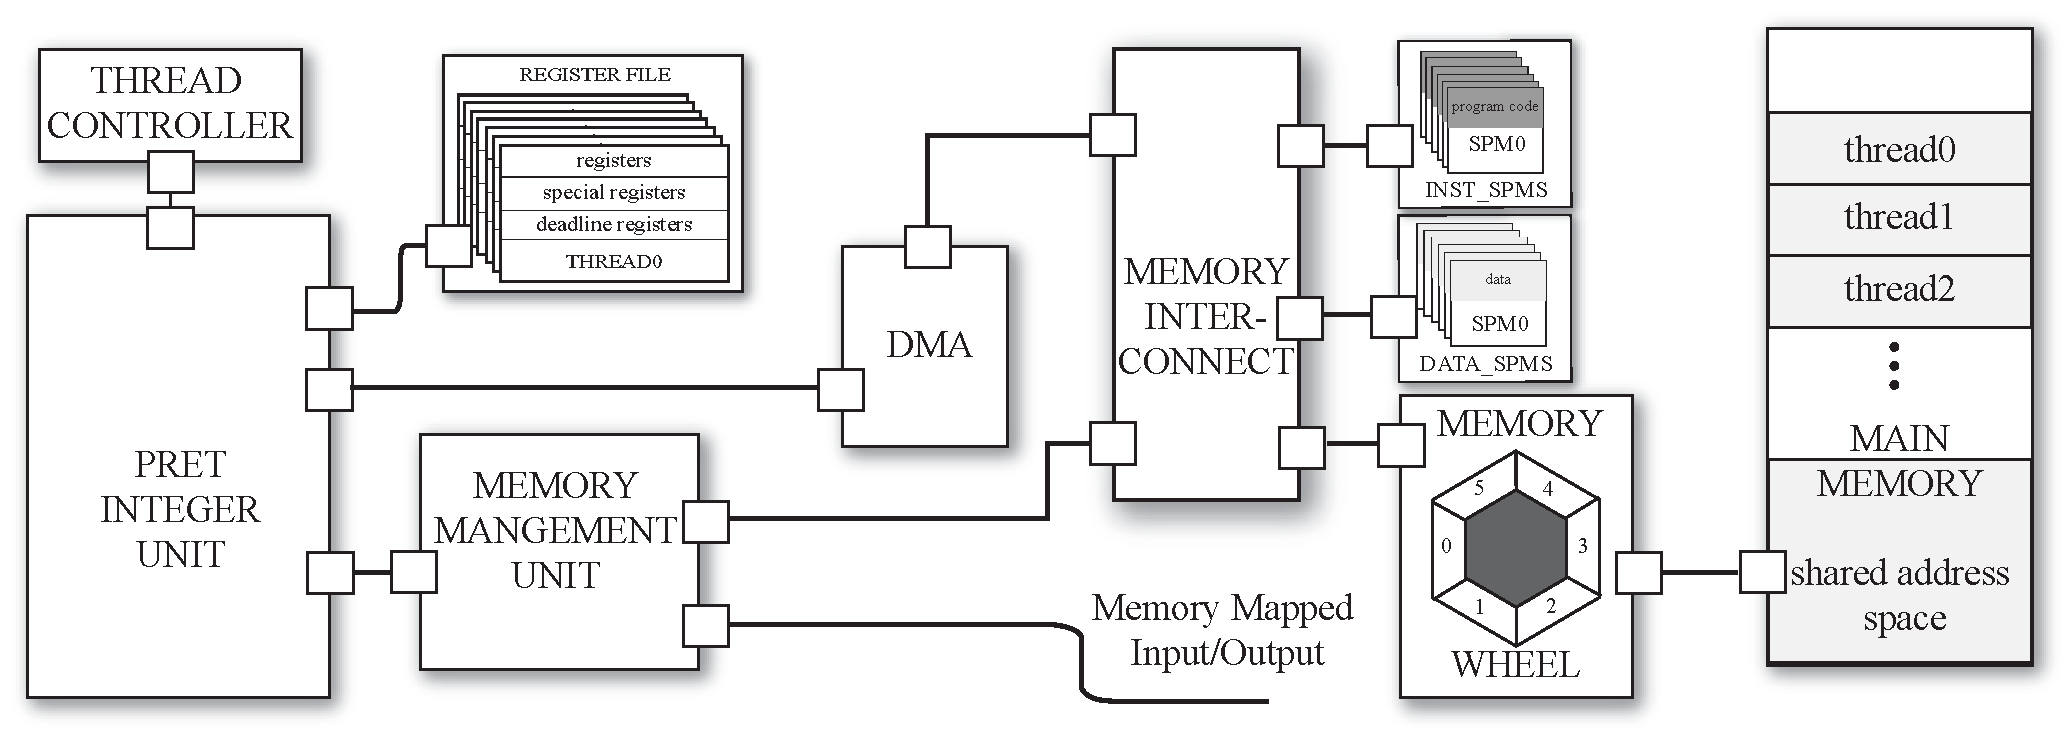
\includegraphics[width=\textwidth]{./images/top_arch.pdf}
%%   \caption{Unit Diagram for PRET Architecture. Reproduced with permission~\cite{pret_cases08}. }
%%   \label{fig:compview}
%%   \end{figure}

\subsection{A Precision Timed Architecture for Embedded Security}
The foundation of time-exploiting attacks exploits the uncontrollable timing variability introduced to programs by underlying the implementation of encryption algorithms.
Software implementations naturally introduce varying run times because of data-dependent control flow paths.
Modern computer architectures create unpredictable execution times by abstracting away hardware optimizations meant to improve average case performance.      
In this section we will present several features of PRET that bring \textit{controllability} over timing to software, eliminating the origin of the attacks.
We will discuss the software extensions that allow timing specification in programs, and the predictable architecture to comply with these specifications.
These two approaches cannot be separated.
A predictable architecture by itself would only ease the feasibility of an attack, and software timing specifications are meaningless if they cannot be met by the hardware. 
By combining both hardware and software solutions, we yield a timing predictable and controllable architecture. 
Thus, by design, PRET prevents leakage of any timing side-channel information, and eliminates the core vulnerability of time-exploiting attacks.

\subsubsection{Controlling Execution Time in Software}
It is extremely difficult to control and reason about timing behaviors in software, even with adequate understanding of the underlying architecture.
Current instruction-set architectures (ISA) have neglected to bring the temporal semantics of the underlying architecture up to the software level.
Thus, architecture designs have introduced clever techniques to improve on average case execution time of the instructions, at the expense of introducing variability in instruction execution time.
These architecture improvements are hidden to the software behind the abstraction of the ISA.   
%The difference in execution time for different paths of the program are often a result of optimizations to the program performance.
This proves to be costly in terms of security, because it uncontrollably leaks timing information which can correlate to the secret key.

In section~\ref{sec:programming_models} we introduced several ISA extensions that add time controlling behaviors to software. 
The extensions provide timing instructions that enable a programmer to have more control of execution time in software.
These instructions do not physically alter processor speed, or modify the execution time of instructions on the architecture.
Instead, they are meant to aid the programmer in dealing with timing variability from data-dependent control flow paths by allowing the programmer to interact with various execution time behaviors in software. 
This includes the ability to specify a desired execution time for code segments, and the ability to detect and handle situations when the execution time exceeds the desired amount.
Specifically in this context, the ability to enforce a minimum execution time for code segments proves extremely useful for mitigating the varying execution speeds exhibited by algorithms or code segments.  
We showed in section~\ref{sec:1dCFD} how the \emph{delay\_and\_set} instruction can be used to synchronize execution and communication of different nodes for an implementation of a real-time 1D-CFD simulation.  
Encryption algorithms can exhibit varying execution time behaviors depending on the bits of the encryption key.
The algorithm follows different execution paths if a particular bit in the key is set or not, allowing attackers to exploit this execution time variance to obtain the key.
By using the timing instructions provided by the PRET architecture, we can mitigate the effects of this, eliminating the exploit causing this timing  attack.  

At the expense of more programming effort, other solutions have been proposed to alter and pad the execution time of different execution paths~\cite{Kocher96timingattacks} to shield against the timing variability of the algorithm. 
At a glance it might seem that the timing instruction are a similar solution to these proposals, however, the principles are inherently different. 
While effective against certain time-exploiting attacks, existing solutions alter the underlying algorithm implementation in attempt to manually pad or distort the execution time. 
These solutions are not only algorithmically specific, but could lead to unnecessarily degrading of the performance of encryption algorithms. 
The timing instructions, on the other hand, allows for a separation of concern between the functionality and timing behavior of the code. 
The programmer can implement the correct functionality of the algorithm, then use timing instructions to regulate its timing behavior.
The subtle difference will be more apparent in section~\ref{sec:rtencrypt-results} when we show two different implementations of the RSA encryption that both use timing instructions to regulate execution time.
One implementation mimics existing execution time padding solutions, and the second implementation uses timing instructions to enforce an overall execution time of the RSA algorithm. 
We present performance comparisons and show that explicit timing control instructions could prove more beneficial than simple execution time padding.  

 %in the results section in section~\ref{sec:rtencrypt-results}. 
% The first implementation mimics the behavior of an existing execution time padding solution by forcing the execution time of all modular exponent operations, regardless of the bit value from the encryption key. 
% This solution leads the execution down the worst-case execution path for any encryption key, which we argue is unnecessarily degrading the algorithm performance.     
% Our second implementation uses statistical analysis on the run time of various input keys in encryption algorithms to determine the enforced execution time of the algorithm. 
% This leads to a modest performance improvement compared to the first approach, as the execution path is not forced down the worst-case path.

%We observe the normal distribution of execution times for the RSA encryption, and chose an execution time that covered roughly 97\% of the keys running in the RSA algorithm.    
%Without modifying the algorithm itself, the timing instructions regulated the execution time to   

%However, because these don't change architectural behavior, 
The timing instructions provide a method to control the timing behavior of a program in software.
However, they do not change the behavior of the underlying architecture.
If the underlying architecture makes the reasoning of execution time difficult, then these instructions become more difficult to use.
Timing instructions alone do not prevent attacks that exploit architectural designs to inject execution time variances~\cite{Percival05cachemissing,branchpredict} and obtain side-channel information. 
We argue that a \textit{predictable} architecture is also required to eliminate timing exploiting attacks.

\subsubsection{Predictable Architecture}
\paragraph {Pipeline}
In order to improve instruction throughput and performance, modern processor architectures implement pipelines to execute multiple instructions in parallel.
This requires handling of pipeline hazards, which are caused by dependencies in instruction sequences. 
Conditional branches are the perfect example -- the pipeline cannot fetch and begin executing the next instruction without knowing which instruction to fetch. 
Since a conditional branch usually takes more than one cycle to resolve, the processor is forced to stall until the branch is resolved. 

Computer architects use clever speculative techniques to mitigate the effects of pipeline hazards and to substantially improve the average-case performance.
For example, branch predictors are used to guess the next instruction needed by the processor for branches~\cite{Grunwald98confidenceestimation}.
This allows the processor to execute instructions speculatively while rolling back only when needed. 
%If the speculation is correct, there is no performance penalty, otherwise, the pipeline is flushed and a new instruction stream is fetched.
While these speculative techniques improve the average-case performance, they introduce several side effects. 
%they result in computer architectures that are \textit{unpredictable}, and \textit{uncontrollable}. 
% \FIXME{Isaac: I find that it would be better to say that these architectures are unpredictable, which make cycle-counting and static prediction of execution times virtually impossible. The uncontrollability has two issues: 1) it's not possible to determine the execution times due to unpredictability, and 2) no method of allowing to do so either (no instructions)}
First, they create \textit{timing variations}.  
Depending on the outcome of its speculation, the processor might need to discard the wrongly speculated work, and re-execute the correct instructions. 
Second, these units are \textit{unpredictable}.
Since these units are shared by all software processes concurrently running on the processor, the states of speculation units are heavily dependent on the different interleaving of processes. 
This means that a process can unknowingly be affected by other processes, since the speculation state is shared between them~\cite{leethreads}.
Because the goal of these speculation techniques is to improve program performance without effort from the programmer, the controls of these speculation units are concealed from the programmer, and cannot be directly accessed in software. 
Thus, these side effects result in \textit{uncontrollable} timing behaviors in the program.

Several Multithreaded architectures enable more opportunities to exploit the uncontrollable timing behaviors.   
Multithreading utilizes thread-level parallelism by introducing multiple hardware threads in the processor.
This allows the execution of another hardware thread during pipeline stalls like branches or memory accesses.
However, typical multithreaded architectures share hardware units effecting execution time between hardware threads, enabling threads to covertly affect other threads execution time.  
The class of Simultaneous Multithreading (SMT) architectures presents an example of this.
Here, the hardware threads share multiple execution units and execute in parallel depending on a hardware scheduler. 
Attackers exploit such designs by running a spy thread that executes concurrently with a thread that implements the encryption algorithm.
This spy thread probes the components shared with the encryption thread~\cite{Percival05cachemissing,branchpredict} by forcefully occupying the shared units and observing when they are evicted by the encryption thread. 
The announcement of this vulnerability caused Hyper-Threading, Intel's implementation of SMT, to be disabled by default in some Linux distributions because of its security risks~\cite{hyperthreadharmfulsite}.
For general purpose applications, these side effects pose insignificant threats, but for security applications, the consequences are uncontrollable sources of side-channel information leakages.

The PREcision Timed (PRET) architecture is a timing predictable architecture  proposed for real-time embedded systems.
As discussed in chapter~\ref{section:pret_thread_pipeline}, PRET employs a thread-interleaved pipeline, a multithreaded pipeline that employs a predictable round-robin thread scheduling policy between the hardware threads every cycle.
Instructions from each thread are predictably fetched into the pipeline every $n$ cycles, where $n$ is the number of hardware threads. 
If $n$ is greater than the number of stall cycles needed for data dependency hazards, then we effectively remove those hazards because the data value is available during the next cycle in which the thread is dispatched. 
For example, if we set $n$ to be the number of stages in the pipeline, then we eliminate the need for any data forwarding/bypassing logic, along with the need for hardware speculation units such as branch predictors.
Most importantly, the hardware threads are temporally isolated, meaning that no threads can affect each others timing behavior.  
Each individual hardware thread maintains their own copy of the processor state (program counter, general purpose registers, stack pointer, etc.), and each hardware thread runs independently with no shared state in the pipeline. 
Because of the simple and transparent thread-scheduling policy, each hardware thread gets dispatched in a predictable way that cannot be affected by other hardware threads. 
Thread-interleaved pipelines allow us to gain higher instruction throughput without the harmful side effects.

\paragraph{Memory System}
The memory system presents another opportunity for attackers to gain side-channel information.
The high clock speed of modern processors combined with the high latency to access main memory results in sometimes hundreds of cycles stalled when the processor needs to access the main memory.
On-chip fast access memories are used to bridge this access latency, creating a \emph{memory hierarchy}.
Caches are \textit{hardware-controlled} fast-access memories that predict and prefetch data from main memory based on temporal and spatial locality of data accesses from the processor.
If the cache control speculation is accurate, then access to data can complete in one cycle, and no stall in the pipeline is required.
However, when a misprediction occurs, data needs to be fetched from the main memory, causing a drastic difference in the access time~\cite{thiele:04:predictable}.
Caches abstract away this memory hierarchy and access latency variation from the programmer by managing the cache contents in the hardware.  
Because threads and processes share the same memory system, attackers can probe the memory access patterns of the encryption process by evicting shared cache lines and observing the timing variation it causes~\cite{Percival05cachemissing}.
This is possible because the memory hierarchy is abstracted away from the programmer, resulting in \emph{uncontrollable} timing behaviors. 
%The cache states are manged in hardware, and shared by all threads and processes.   

PRET utilizes scratchpads memories (SPM) instead of caches in its memory hierarchy.  
SPMs are fast access memories controlled by software. 
SPMs use less power and occupy less area~\cite{Banakar2002} because no speculation logic is needed. 
SPMs occupy a distinct address space, which exposes the memory hierarchy to the programmer, instead of abstracting it away like caches.  
The allocation of data between memory and SPM is done with explicit instructions, either at compile time by the compiler or manually by the programmer.
This gives the software control over memory access latencies, and provides a predictable execution time of the program.
The performance of SPMs vary based on the data access patterns of the application, but since the control is in software, it is possible to tune the allocation scheme to achieve even better performance than a generic cache for specific applications. 
There are abundant ongoing research on allocation schemes and methods for optimizing the performance of SPMs~\cite{avissar2002oma,Bandyopadhyay:EECS-2006-105,Patel:EECS-2008-115,WCETSPM,compilerSPM}. 
SPMs can be found in the Cell processor~\cite{cellproc}, which is used in Sony PlayStation 3 consoles, and NVIDIA's 8800 GPU, which provide 16KB of SPM per thread-bundle~\cite{8800gpu}.
Although this comes at the cost of more programing effort, but it is not uncommon to see platform specific tuning of software for performance purposes. 
For example, high performance parallel algorithms are often fine tuned to work on block sizes depending on the cache size and replacement policy of the platform, and re-tuned when running on different platform.

For security purposes, the scratchpad on PRET is configured to provide each hardware-thread a private scratchpad region so the scratchpad contents cannot be modified or monitored by spy threads on running another hardware thread.    
This prevents shared resource time-exploiting attacks on the fast access memory across hardware threads.
Even if an encryption process is sharing a hardware thread with another process, the contents of the scratchpad is controlled in software or statically compiled in by the compiler.
The thread managing supervisor code can manage the contents on the scratchpad before the processes are scheduled and unscheduled, preventing a spy process from affecting the execution time of the encryption process. 
Clearly, the edge that SPMs give over conventional caches is their \emph{controllability} in software, thus preventing unwanted timing side-effects from attackers and spy threads, even though the SPM is shared by software processes.
%If caches must be used, hardware additions to the cache
%Partition locked caches, which allows software processes to to lock cache lines which have proven successful against cache attacks~\cite{cachepartition}, can be implemented. 

Although no known attacks have exploited main memory access, typical DRAM controllers also result in variable memory access latencies, and are shared amongst all threads and processes within the system. 
A predictable DRAM controller is designed and interfaced with the thread-interleaved pipeline of PRET to provide predictable memory access latencies to all threads. 
The DRAM controller privatizes DRAM bank resources to remove bank conflicts and fully utilize bank level parallelism on the DRAM.  
Each hardware thread in the thread-interleaved pipeline is mapped to a privatized DRAM bank resource.
On the backend, the bank resources are accessed in a round robin order fashion, to remove temporal interference between accesses to the bank resources.
All memory accesses from the hardware threads are isolated from each other, removing any possibilities of cross-thread side-channel attacks from the shared memory controller.
The DRAM memory access latencies are decoupled from the data access patterns, thus, even processes on the same hardware thread that access the same bank resources cannot alter each others execution time in attempt to gain side-channel information.  
More details on the PRET DRAM controller is presented in section~\ref{sec:pret_dram_controller}.

We acknowledge the many efforts to counteract timing attacks with algorithm rewrites to control and balance the run time of the algorithm. 
These efforts while successful, are ad-hoc, counteracting specific attacks without prevention of others.
Without tackling the origin of time-exploiting attacks, we believe that more exploits will eventually be discovered, attacking the \emph{uncontrollable} execution time variation caused by the shared resources of hardware or software control flow.  
The PRET architecture is designed to ensure repeatable and predictable timing behavior of programs by providing control of timing properties in software and a predictable architecture that provides temporal isolation for hardware threads and processes.
PRET is impenetrable known attacks such as branch predictor attacks~\cite{Onur07predictingsecret}, cache attacks~\cite{Percival05cachemissing} or other attacks on the pipeline~\cite{2009-x86timing}.
The more importantly, the predictable architecture design removes the root cause of time-exploiting attacks -- the \emph{uncontrollable} timing variations caused by unpredictable hardware components or software control flows.     

\subsection{Case Studies}
\label{sec:rtencrypt-results}
In the following section we will show results of two encryption algorithms running on PRET. 
All experiments are run on the cycle accurate simulator of the PRET architecture described in~\cite{pret_cases08}.
The simulator implements the SPARC v8 instruction set, and employs six threads on a six stage thread-interleaved pipeline.
Programs are written in C and compiled using a standard gcc cross compiler from Gaisler research labs~\cite{GAISLER}.
This PRET implementation implements a simple processor extension inspired by Ip and Edwards~\cite{ip2006processor} that adds timing instructions to the ISA.
To be consistent with the terminology used in~\cite{ip2006processor}, we call this instruction the \textit{deadline instruction}.
This deadline instruction has similar semantics to the \emph{delay\_and\_set} instruction introduced in section~\ref{sec:programming_models}. 
It first ensures the previous deadline specified is met, then sets the deadline for the next instruction sequence.
The deadline instruction specifies time in units of thread cycle, which is a thread's perceived cycle.
  
% The deadline instruction is used to load values into a special set of registers, called the \textit{deadline registers}. 
% In ~\cite{ip2006processor}, these registers are decremented each clock cycle in hardware, and act as hardware cycle counters. 
% Whenever the processor executes a deadline instruction, it first checks the corresponding deadline register's contents. 
% If it is zero, then the value specified in the instruction is loaded into the register, and the program continues. 
% If not, the processor replays this instruction until the value reaches zero. 
% Figure ~\ref{fig:timing_want} shows a simple illustration of what the deadline instructions look like.
% By enclosing instruction blocks within two deadline instructions, we can specify that the enclosing code block should run for x or y cycles.
% In ~\cite{ip2006processor}, this instruction was implemented for a single cycle processor. 
% PRET extended this instruction to be used in a multi-threaded pipeline architecture. 
% We will later show a more concrete example of how this instruction is extended for PRET.

% \begin{wrapfigure}[13]{l}{.4\textwidth}
%   \centering
%   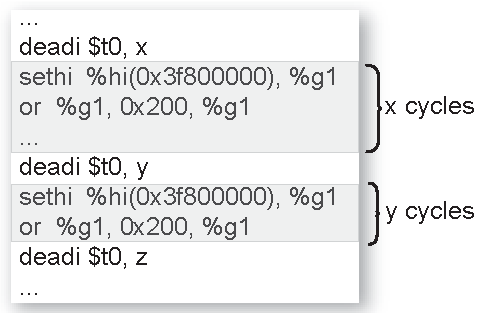
\includegraphics[scale=.7]{./figs/RTencrypt/timing_want.jpg}
%   \caption{A method to express timing requirement in software.}
%   \label{fig:timing_want}
% \end{wrapfigure}

%%Talk about the different in decrementing deadlines in PRET vs
%%original paper?
%This instruction allows a user to specify the execution time of the code enclosed within the deadline instructions. 


% \subsubsection{Timing instructions on PRET}
% 
% \begin{wrapfigure}[11]{r}{.4\textwidth}
% %\begin{SCfigure}
%   \centering
%   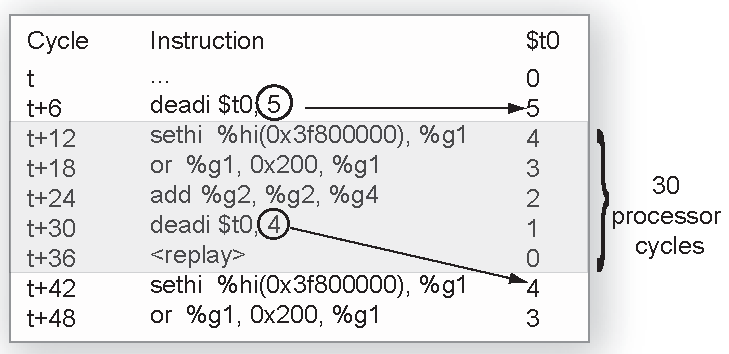
\includegraphics[scale=.53]{./figs/RTencrypt/timing_instructions.jpg}
%   \caption{A simple example using deadline instructions on PRET}
%   \label{fig:deadline}
% %\end{SCfigure}
% \end{wrapfigure}
% 
% Since PRET has multiple hardware threads, each hardware thread contains its own set of deadline registers, which are decremented every time an instruction from that thread is fetched into the pipeline.
% Specifically, PRET has six hardware threads, so each hardware thread's deadline registers are decremented every six processor cycles.
% Figure~\ref{fig:deadline} shows a concrete example of the execution of one thread on PRET using the deadline instruction.
% The three instructions enclosed between the deadline instructions take exactly 30 cycles to execute. 
% \textit{\$t0} shows the contents of deadline register 0. 
% The processor cycle is shown to the left of the instruction.
% When the first deadline instruction is executed, the instruction will simply load 5 into deadline register 0 and continue because the value of \emph{\$t0} is currently 0.
%  When the second deadline instruction is executed, since the value of \emph{\$t0} is not decremented to zero yet, this instruction will be replayed. 
% Only at \emph{t+36} cycles will the value 4 be loaded into deadline register 0.
% This ensures that the code enclosed will take 30 cycles to execute, as specified in the first deadline instruction. 
% We will show two real-world examples of using deadline instructions with encryption algorithms later in the case study section.

\subsubsection{RSA Vulnerability}

The central computation of the RSA algorithm is based primarily on modular exponentiation. 
This is shown in algorithm~\ref{alg:rsa}.
Of the inputs, $M$ is the message, $N$ is a publicly known modulus, and $d$ is the secret key.  
Depending on the value of each bit of $d$ on line 4, the operation on line 5 is either executed or not. 
This creates variation in the algorithm's execution time that is dependent on the key, as mentioned in \cite{Kocher96timingattacks}.

\begin{minipage}[h]{0.4\textwidth}
  \scriptsize
\begin{algorithm}[H]
\label{alg:rsa}
  \LinesNumbered
  \SetAlgoVlined
\KwIn{M, N, d = $(d_{n-1}d_{n-2} . . . d_{1}d_{0})$}
\KwOut{S = M$^{d}$ mod N}
S $\leftarrow$ 1 \\
\For{j = n - 1 $. . .$ 0} {
S $\leftarrow$ S$^{2}$ mod N \\
\If{d$_{j}$ = 1} {
S $\leftarrow$ S $\cdot$ M mod N
}
\textbf{return} S
}
\caption{RSA Cipher}
\end{algorithm}
\end{minipage}
\begin{minipage}[h]{0.6\textwidth}
  \scriptsize
\begin{algorithm}[H]
  \LinesNumbered
  \SetAlgoVlined
\KwIn{M, N, d = $(d_{n-1}d_{n-2} . . . d_{1}d_{0})$}
\KwOut{S = M$^{d}$ mod N}
S $\leftarrow$ 1 \\
\For{j = n - 1 $. . .$ 0} {
/* 110000 is 660000$\div$6 cycles, since deadline registers are decremented every 6 cycles.*/ \\
\textbf{dead(110000);}\\
 S $\leftarrow$ S$^{2}$ mod N \\
\If{d$_{j}$ = 1} {
S $\leftarrow$ S $\cdot$ M mod N
}
\textbf{dead(0)}; \\
\textbf{return} S
}
\caption{RSA Cipher with deadline instructions}
\label{alg:rsa_w_dead}
\end{algorithm}
\vspace{2mm}
\end{minipage}


%Our analysis of the algorithm demonstrated that a significant portion of the variation in the algorithm's execution time could be attributed to the branch in the loop above.  
When the reference implementation of RSA (RSAREF 2.0) was ported to the PRET architecture, single iterations of the loop varied in execution time almost exclusively due to the value of d$_{j}$, which is the j$^{th}$ bit of the key. 
The triangle points in figure \ref{fig:modexp} show the measured run time of each iteration in the for loop (lines 2--6) in algorithm \ref{alg:rsa}. 
Each iteration took approximately either 440 or 660 kilocycles, with very little deviation from the two means.
As a simple illustration, we can fix the execution time of each iteration in software  by adding deadline instructions in the body of the loop as shown in algorithm~\ref{alg:rsa_w_dead}. 
When enclosed with deadline instructions, the execution time of each iteration is uniform, and the bimodality of the execution time is completely eliminated. 
The x points in figure \ref{fig:modexp} show the measured time of each iteration after adding deadline instructions; they are simply a straight line.

\begin{figure*}[h]
\centering
\subfigure[Run time of Modular Exponent operation] {
  \includegraphics[width=0.48\textwidth]{./figs/RTencrypt/ModExp.pdf}
  \label{fig:modexp}
}
%\quad
\subfigure[Run time of RSA operation]{
  \includegraphics[width=0.48\textwidth]{./figs/RTencrypt/RSA.pdf}
  \label{fig:rsa}
}
\caption{RSA Algorithm}
\end{figure*}



%We see that all iterations took exactly the same amount of time. 
%These results seem obvious, but reveal the power of software-controlled execution time. 
%Now algorithms that require constant run time can easily be specified in software.  
%Additionally, placing deadline instructions in this loop completely eliminates the vulnerability mentioned in Kocher's\cite{Kocher96timingattacks} classic timing attack paper. 
We observe the large-scale effect of this small change on the whole encryption in figure~\ref{fig:rsa}, where RSA was run fifty times using randomly generated keys.
Without the deadline instructions (triangle points), different keys exhibit significant diversity in algorithm execution time.  
With the deadline instructions added within the modular exponentiation loop (circle points), the fluctuation is dramatically reduced to almost none. 
The remaining small variations result from code that is outside of the modular exponentiation loop, which is not influenced by the actual key.
From figure ~\ref{fig:rsa} we can see that this small variation  is not significant enough to correlate the total execution time and the key.  

% Although it seems we could have achieved a similar effect if we simply forced the algorithm to carry out the extra operation every iteration, there is a subtle difference.
% As mentioned in~\cite{Kocher96timingattacks}, always carrying out the extra multiplication operation does not make the implementation run at constant time, and timing characteristics from the squaring operation can still be exploited. 
% However, constant run time is guaranteed for code blocks enclosed within the deadline instructions, which in our case includes both the multiplication and squaring operations for each iteration.
% This simple example demonstrates the difficulty of controlling execution time using software techniques, and how straightforward it is to do so using deadline instructions. 
% This is a simple example demonstrating the concept of the deadline instruction.  
% However, for more complex algorithms, the changes required to create constant execution time might not be as obvious.
% In those situations, deadline instructions provide a straightforward mechanism to control the execution time of the algorithm.

%Although this method makes RSA secure against timing attacks, it does incur a notable performance penalty because we always run the algorithm near its worst-case execution time.
Without explicit control over timing, any attempt to make an algorithm run at constant time in software would involve manual padding of conditional branches.
This forces the algorithm to run at the worst-case execution time, similar to what we've showed.
As a result, although this makes the encryption algorithm completely secure against time-exploiting attacks, they are not adopted in practice because of this overhead.
Nevertheless, with control over execution time, we will show that running encryption algorithms in constant time does not necessarily require it to run at the absolute worst-case execution time.

%smarter techniques with deadline instructions can be used to achieve better performance while still being secure.
%Although the vulnerability is removed, readers will have noticed that an overhead was induced in this simple example. 
%The reason for the overhead is apparent, and mentioned above. 
% This overhead is not a result of the deadline instruction itself. 
% When we added the deadline instructions to the inner most loop of the modular exponentiation, in order to completely remove the vulnerability from RSA, we set the execution time of each loop iteration to always equal the execution time as if the extra operation was carried out. 
% As a result, the overall execution time will be the worst case execution time of the algorithm, as if our key was all bits of 1. 
% That is the overhead we see in figure~\ref{fig:rsa}. 
% This solution is effectively the same as timing equalization \textcolor{red}{(FIXME: add citation [do we really need one? or is this where a paper that talks about what timing equalization is would go?])} of algorithms, which now require little effort because timing can be controlled in software. 
\subsubsection{An Improved Technique of using Deadline Instructions} 
\begin{wrapfigure}[16]{r}{.45\textwidth}
%\begin{SCfigure}
\vspace{-5mm}
  \centering
  \includegraphics[scale=.60]{./figs/RTencrypt/Distro.pdf}
  \caption{Run time distribution of 1000 randomly generated keys for RSA}
  \label{fig:distro}
%\end{SCfigure}
\end{wrapfigure}

It is expected that the distribution of RSA run times will be normal over the set of all possible keys~\cite{Kocher96timingattacks}. 
Figure~\ref{fig:distro} shows the run time distribution measured for one thousand randomly generated keys. 
A curve fitting yields  a bell shaped curve formed from the run time distribution of all keys.
This means that the execution time of approximately 95\% of the keys will be within $\pm$2 standard deviations of the mean, and the worst-case execution time will be an outlier on the far right of this curve. 
Our previous example fixed the execution time of all keys to be \textit{roughly} at this far right outlier.
An improved technique capitalizes on this distribution of run times to improve performance.

First, instead of enclosing the loop iterations of the modular exponentiation operation, we enclose the whole RSA operation with deadline instructions. 
Now the deadline instructions are used to control the overall execution time of the RSA operation.
Note that we could have done this for the previous example as well to fix the execution time to be \textit{exactly} the worst-case, always. 

For RSA, key lengths typically need to be longer than $512$ bits to be considered cryptographically strong~\cite{redhatadminguide}. 
This gives roughly $2^{512}$ possible keys, which is far more than needed for most applications.
Suppose we are able reduce the key space the application covers --
instead of using $100\%$ of the keys, we refine our encryption system to only assign $97\%$ of all possible keys. Namely, the subset of keys whose RSA execution times fall on the left of the $+2$ standard deviation line on the curve.
Statistically, the keys that lie outside of $\pm 2$ standard deviation are the least secure keys anyway, since it is easier for time-exploiting attacks to distinguish those keys. 
%Then, we can reduce the value specified in the deadline instruction enclosing the whole RSA operation instead of using the absolute worst-case execution time pushed up by the far right outlier.
By doing so, we reduce the execution time of the encryption algorithm because we know that keys that are right-side outliers will not be used. 

With timing control in software, we can take advantage of this information by simply reducing the value specified in the deadline instructions enclosing the whole RSA operation. 
The square points in figure~\ref{fig:rsa} show the results of using deadline instructions in this way. 
We re-ran the same fifty keys from the previous section, and enclosed the whole operation with deadline instructions that specified the run time at +2 standard deviations from the bell curve we obtained.
We can see that, compared to the previous results that fixed the execution time of each key to take  the worst-case time (circle points), we clearly reduced the overhead while still running in constant time. 
By taking the run time difference between executions with and without deadline instructions, we obtained the overhead introduced for each of the keys with run time below 2 standard deviations (97.9\% of keys in our case) within the one thousand key set in our experiment. 
This calculation reveals that by merely reducing the key space by 3\%, running the encryption with optimized deadline instructions only introduced an average overhead of $2.3\%$ over all the keys we measured. 
All this while still being completely immune to time-exploiting attacks.
This is virtually impossible to achieve without explicit timing control, which illustrates the value of decoupling timing control and functional properties of software. 

%When running on PRET, we measured an average overhead of $11\%$ over the one thousand keys in the when we controlled the execution time of each iteration within the modular exponentiation operation.


\begin{figure*}[h]
\centering
\subfigure[Distribution of 1000 DSA keys ] {
  \includegraphics[width=0.48\textwidth]{./figs/RTencrypt/DSA_Distro.pdf}
  \label{fig:dsamodexp}
}
%\quad
\subfigure[Run time of 100 DSA operations]{
  \includegraphics[width=0.48\textwidth]{./figs/RTencrypt/DSA.pdf}
  \label{fig:dsa}
}
\caption{Digital Signature Standard Algorithm}
\end{figure*}

\subsubsection{Digital Signature Algorithm}
Kocher's~\cite{Kocher96timingattacks} original paper mentioned that Digital Signature Standard~\cite{dss} is also susceptible to timing attacks. 
Thus, to further illustrate our case, we ported the Digital Signature Algorithm from the current OpenSSL library (0.9.8j) onto PRET.
We used the same method mentioned above to secure this implementation on PRET.
Figure~\ref{fig:dsamodexp} shows the distribution of DSA run time for one thousand keys. It also shows a normal distribution.
Then, we randomly generated another one hundred keys, and measured the run time with and without deadline instructions, which we show in figure~\ref{fig:dsa}.
We can see clearly that the run time with deadline instructions is constant, and any time-exploiting attack is not possible. 

%we can set different values for the deadline instruction depending on the application's needs to yield a balance between security and performance. 
% Another possible use of deadline instructions is to implement execution time blinding. 
% We can set the execution time  of the encryption operation to be a truly random value between $\pm$2 standard deviations of the total run time. 
% Whenever the value of the deadline instruction is less the actual run time of the algorithm, the algorithm will take its normal execution time. 
% However, if the value of the deadline instruction is more than the run time, then the algorithm will run at the time specified by the deadline instruction. 
% Since the deadline instruction value is random, it detaches the correlation between the key and the run time of the encryption. 
% This can also improve the average performance.

%Simply by running on PRET, RSA is not only immune to cache attacks and branch predictor attacks, both of which can be significant dangers to RSA\cite{branchpredict,Percival05cachemissing}, but also to potential unknown timing attacks targeting the unpredictability of the architecture. 

Currently, we do not know of any work that correlates the key value with run time for different encryption algorithms. 
However, with the ability to control execution time in software, such a study would be extremely valuable.
Figures~\ref{fig:distro} and~\ref{fig:dsamodexp} show that RSA and DSA follow a normal distribution.  
Thus, from the algorithm, we postulate that by simply counting the $1$ bits in the key should be sufficient to distinguish the $95\%$ of secure keys before assigning. 
Note that no change to the encryption algorithm itself is needed, but only the key assignment process.
Since we can adjust the execution time in software, we can tune the performance of each application based on the application size, key bit length and performance needs.
All this can be done while maintaining complete immunity against time-exploiting attacks.

Note that there are several other software techniques specific to encryption algorithms that successfully defend against timing attacks. 
Our work does not lessen or replace the significance of those findings.
Instead, we can use traditional noise injection defenses on PRET as well.
For example, if reducing the key space is not possible for some applications running RSA then RSA with blinding can be ran on PRET. 
By simply running on PRET, the encryption algorithm is also secure against shared hardware resource attacks such as caches, and branch predictors. 
Other encryption algorithms that do not have software techniques or solutions readily available to counteract timing attacks can easily use the deadline instructions provided by PRET to achieve security against timing attacks.

% \section{Future Work}
% While a deadline instruction set for the worst case execution time bestows complete immunity to timing attacks, it also places overhead on virtually every execution, which may be substantial depending on the application.  Lowering the minimum time, even randomly, gives some information to an attacker, especially if there is no limitation on the number of executions the attacker may observe.  A mathematical examination of the risk involved in a reduced execution time would enable the programmer to decide what tradeoff of risk and execution delay was appropriate for the application, or appropriate in general.  For example, reducing the potential key space to a tenth of all possibilities would most likelyside-channel be an acceptable trade for faster execution, while reducing it to a billionth of all possibilities probably would not be acceptable.

% On another note, the PRET architecture as it stands is vulnerable to power attacks.  By doing very little and drawing less power while waiting for deadlines to expire, timing attacks are basically converted into a subset of power attacks.  This is unacceptable for consumer applications such as set-top boxes, where power draw can be easily measured.  Modifying the architecture to spend energy while waiting would prevent such attacks.  Depending on the implementation of the power-draining system, it might even be extended to prevent most other power attacks as well by adding another power sink to that required for useful work.

\subsection{Conclusion and Future Work}
Side-channel attacks are a credible threat to many cryptosystems.  
They exist  not just because of a weakness in an algorithm's mathematical underpinnings, but also from information leaks in the implementation of the algorithm. %The inability to control timing properties is what directly leads to side channel attacks.
In particular, this paper targets time-exploiting attacks, and lays out a means of addressing what we consider the root cause of such attacks: the lack of \textit{controllability} over the timing information leaks.
%Although numerous efforts have been put to discovering and counteracting these attacks, it seems that only more vulnerabilities are being discovered. 
% Without secure hardware, software cannot be considered truly secure.  
% Some stopgap measures are implementable in software, but rarely are they a guaranteed fix.
%that originate from the \textit{unpredictability} of the underlying hardware architecture.
As an architecture founded on predictable timing behaviors, PRET provides timing instructions to allow timing specifications in software. 
In addition, PRET is a predictable architecture that guarantees removes timing interference through a thread-interleaved pipeline with scratchpad memories for each hardware thread, and a predictable DRAM memory controller.
This eliminates the shared states in the architecture that create uncontrollable timing interference, exploited by attackers. 
Through a combination of hardware and software techniques, PRET gives control over the timing properties of programs, which effectively eliminates time-exploiting attacks. 

We demonstrate the application of these principles to known-vulnerable implementations of RSA and DSA, and show that PRET successfully defends against time-exploiting attacks with low overhead. 
Our work does not undermine the significance of any related work, which have mostly been specific to certain attacks.
PRET does not target a specific encryption algorithm, because it can be used in combination with these partial solutions on specific encryption algorithms, as well as provide a complete defense for other encryption algorithms which are less researched upon.

Besides time-exploiting attacks, there are other side-channel attacks that are legitimate threats to encryption algorithms such as power, and fault attacks.
We plan to continue to investigate PRET's effectiveness in defending against them. 
We conjecture that the thread-interleaved pipeline used in PRET can potentially help defend against power attacks because the power measured from the processor now includes significant interference from the execution of other hardware threads in the architecture.  
%Currently, PRET is only implemented as a software simulator, but as PRET moves to FPGA implementations, we can further evaluate its effectiveness in defending against power attacks.
%If our conjecture is correct, then PRET with fault tolerant techniques could potentially be a complete solution against several major side-channel attacks.  

\chapter{Related Work}
\label{chapter:related}
Intro text here

\section{Related Section Header}
\label{sec:related_sec_1}

Fig.~\ref{fig:placeholder_related} shows an image

\section{Related Section Header 2}
\label{sec:related_sec_2}

Here is another header


\begin{figure}
\begin{center}
\vspace{-32pt}
\includegraphics[scale=.45]{figs/placeholder}
\end{center}
\vspace{-12pt}
\caption{Image Placeholder}
\label{fig:placeholder_related}
\end{figure}


\chapter{Conclusion and Future work}
\label{chapter:summary}
In order to propel the use of CPS for safety critical systems, we contend that changes must be made to conventional abstraction layers to introduce ``time'' as its first class citizen.
In this thesis we focused on the ISA abstraction layer and below.  
We explored instruction extensions to the ARM ISA in order to bring temporal semantics to the programs from the ISA.  
We also presented the precision timed ARM (PTARM), an implementation of a PRET machine, in order to provide a timing predictable and composable platform for deterministic execution time.  

To bring temporal semantics to the ISA abstraction layer, we presented a few instruction extensions to the existing instruction set. 
The instructions operate on a platform clock that is synchronous with the execution of instructions. 
The instructions extensions allow programmers to specify the timing properties of program segments, and throw hardware exceptions when the timing specifications are not met.
In this way, our instruction extensions does not over constrain the temporal semantics of the ISA, and still allows architecture innovation to improve program performance. 
These extensions allows programmers to begin reasoning about temporal properties of the programs independent of the underlying execution platform, provided that the ISA is faithfully implemented.

PTARM exploits thread-level parallelism for performance by employing a predictable thread-interleaved pipeline. 
This removes the unpredictability when handling pipeline hazards, and provides temporal isolation for all hardware threads within the pipeline.
PTARM uses scratchpads instead of caches to expose the memory hierarchy, which enables simpler and tighter WCET analysis. 
With a bank privatized DRAM controller, PTARM gives predictable memory access latencies to the DRAM for each hardware thread, and preserves temporal isolation for each hardware thread that accesses the DRAM as a shared resource.
We show that PTARM offers both timing predictability and composability, equipping CPS platforms the tools to interact with physical processes deterministically.

We also demonstrated the the benefits of a PRET machine in the context of a real-time engine fuel rail simulator and embedded security.
For simulating engine fuel rails in real time, we showed a platform that uses multiple PTARM cores which communicate through local shared buffers. 
The predictable timing of PTARM enables a software timing based synchronization between the cores that is implemented with the timing instruction extensions.  
In the context of embedded security, the underlying architecture implementing encryption algorithms are susceptible to timing side-channel attacks, which allows attackers to exploit the uncontrollable execution time variance to derive the key. 
We show that with a predictable architecture and controllable timing properties of the program, we not only defend against all timing side-channel attacks, but eliminate its root cause. 


Several open challenges and questions were mentioned in this thesis, which provides grounds for future research opportunities.  
First, we continue to explore the formalization of the timing extensions to the ISA. 
The introduction of temporal semantics in the ISA should be platform independent; our implementation in PTARM merely open up opportunities for further experimentation and research. 
Nailing down the formal semantics of each extension is key to a consistent meaning of ``time'' independent of the underlying platform implementation. 
Second, how a predictable pipeline and memory controller handles external interrupts and I/O devices still remains an open question.
With the plethora of complex interfaces and protocols for modern high speed I/O interactions, typical I/O controllers are implemented in hardware.
However, we envision a predictable architecture with precise timing control to enable software implementations of protocols typically implemented in hardware. 
This can enable flexibility and more efficient design effort, leading to faster time-to-market and more feature rich designs.        
Third, the interfacing with a timing predictable bus or interconnect can give means to implementing a predictable multicore architecture.
We showed a primitive multicore implementation of PRET cores when simulating engine fuel rails in real time.
However, as communication schemes get more complex, how synchronization and communication of multiple PRET cores is done remains an open question and research challenge. 

It is important to understand that we are not proclaiming that all dynamic behavior in systems are harmful.
However, the dynamic behavior must be controllable and predictable. 
For example, dynamically scheduling hardware threads in the architecture causes uncontrollable timing interference because the triggering of thread switches is hidden from, and cannot be explicitly controlled by, the programmer.
We argue that only by achieving predictability in the architecture and platforms can we begin to reason about more dynamic behavior in software.
With a predictable architecture and the introduction of temporal semantics in the ISA, we hope to provide a deterministic foundation to enable larger and more efficient designs of cyber-physical systems. 



%backup the six stage details 
%\appendix
%\chapter{PTARM 6 stage}
%\section{PTARM 6 stage Architecture}
\begin{figure}
  \vspace{-20pt}
  \begin{center}
    \includegraphics[scale=.6]{figs/ptarm_pipeline_six_stage}
  \end{center}
  \vspace{-20pt}
  \caption{Block Level View of the PTARM 6 stage pipeline}
  \label{fig:ptarm_pipeline_six_stage}
\end{figure}

The pipeline of PTARM implements a thread-interleaved pipeline for the ARM instruction set.
PTARM is written in VHDL and targets Xilinx Virtex-5 Family FPGAs, thus a the design decisions made tailored the PTARM architecture towards optimizing the design for the Xilinx V5 FPGA.
It has a 32 bit datapath and consists of a six stage pipeline and can support a minimum of six threads interleaving through the pipeline.
The pipeline can be clocked up to $180MHz$ on a Virtex-5 lx110t FPGA.  
Figure~\ref{fig:ptarm_pipeline_five_stage} shows a block diagram view of the pipeline. 
The multiplexers within the pipeline have been omitted in the figure for a simplified view of the hardware components that make up the pipeline.
There contains multiple copies of the Program Counter(PC), Thread States, and Register File, which are not shown in the figure.
Most of the pipeline design follows a typical Hennesy and Patterson\todo{citation} 5 stage pipeline, but the thread interleaved pipeline also allows us to strip away the branch predictor and the data forwarding logic used to handle data-hazards.
The six stages in the pipeline are -- Fetch, Decode, Shift, Execute, Memory, Writeback.
We will briefly describe the functional blocks of each stage, and later show how most instruction types are implemented in the pipeline.  
%TODO: Talk about register file, 3 read and 1 write port

The fetch stage of the pipeline selects the correct PC according to which thread is executing, and passes the address to instruction scratchpad.
A simple $Log(n)$ bit upcounter is used to keep track of which thread current to fetch.  
At this point we assume the source code fits entirely on the instruction scratchpad.
Later when we present the memory hierarchy of PTARM we will discuss further about the implications of larger code bases.
Once the instruction is received from the scratchpad, it goes through a register address decoder to quickly determine what bits to send to the register.
Typical RISC instruction sets such as MIPS have encoding of instruction bits where the register operands have a fixed location for all instruction types.
Thus, once the instruction is received from instruction memory, the selected bits can be propagated as addresses to the register file. 
In the ARM instruction set however, not all instruction encoding have the register addresses at the same location. 
Thus, we insert in a simple and small logic block for a quick decoding of register addresses.
%Todo: Add more description of the logic block? 

The decode stage of the pipeline consists of the pipeline controller which does the full decoding of instructions and sets the correct pipeline signals to be propagated down the pipeline. 
Typically the controller needs to know the current instructions in the pipeline to detect the possibility of pipeline hazards.
However,in a thread-interleaved pipeline, other instructions in the pipeline belong to other threads, thus the controller logic is greatly simplified. 
It simply decodes the instruction to determine the correct signals to send to the data-path and multiplexers down the pipeline. 
These signals get propagated down the pipeline stages, and they control the execution units to ensure the correct actions are taken, and signal the multiplexers to select the correct data operands.  
Because most of ARM instructions are conditionally executed, the pipeline controller also checks the condition bis to determine whether the instruction is to be executed or not.  
The PC Adder is almost just a simple adder that increments the PC. 
The only addition is instead only outputting an address incremented by four, it outputs two addresses, the PC incremented by both four and eight. 
The address calculation of ARM branch instructions add the offset to PC+8, instead of just the current PC, so we need to store the additional PC offset of eight in case of branch instructions.
The Timer logic block is a hardware counter clocked to the processor clock which is used to implement the timing instructions mentioned in chapter~\ref{chapter:programming_models}.
The Timer counts time in nanoseconds, and it's hardware logic does not reside in the decode stage. 
The time value however is latched in the decode stage as the subsequent stages use it for timer manipulation, so in figure~\ref{fig:ptarm_pipeline_five_stage} we include it in the decode stage.
We will discuss in more detail how the timing instructions are implemented later in this chapter. 

The shift stage of the pipeline is the additional stage on top of a conventional five stage pipeline. 
The ARM ISA data-processing instructions include shifter bits and even a shifter operand for data-processing register shift instructions to shift the operands before the logical or arithmetic operations.
Thus, an extra 32 bit shifter is included to shift the operands before the execution stage. 
The Load/Store Multiple Offset logic block is used to calculate the offset of load/store multiple instructions.
The load/store multiple instruction uses a 16 bit vector to represent each of the 16 general purpose registers.
The bits that are set in that bit vector represents a load/store on that register.
The an offset is added to the base memory address for the instruction, and that offset depends on how many bits are set. 
Thus, the load/store multiple offset logic block does a bit count on the bit vector and adjusts the offset to be passed into the ALU for load/store multiple instructions.
We will later describe in detail how the load/store multiple instructions are executed within the pipeline.
The timer adder logic block is a 32 bit add/subtract unit. 
Since time is represented in 64 bit values, we add an additional 32 bit add/subtract-er so the execution stage doesn't need to incorporate a 64 bit ALU.

The execute stage simply just contains the 32 bit ALU that can do both logical and arithmetic operations. 
The memory stage interacts with the data scratchpad and memory controller, and the write back stage writes the correct data back to the registers and hardware thread states.

The floating point hardware units are pipelined floating point computation units generated with the Xilinx Coregen tool. 
 
%TODO: Memory Hierarchy
\section{Instruction Implementations}
In this section we will go into more details about how each instruction type is implemented and how the hardware blocks shown in the previous sections are used.
We will go through different instruction types and also discuss the timing implications of our implementation. 
We will summarize with a table with all instructions and the cycle count it takes to execute them.   
\subsection{Data-Processing}

\subsection{Branch}
\begin{figure}
  \vspace{-20pt}
  \begin{center}
    \includegraphics[scale=.6]{figs/branch_pipeline_implementation}
  \end{center}
  \vspace{-20pt}
  \caption{Branch Instruction Execution in the Ptarm Pipeline}
  \label{fig:branch_pipeline_implementation}
\end{figure}
Branch instructions in the ARM can conditionally branch forward or backwards by up to 32MB. 
Because the general purpose register 15 is the PC, any write to R15 is also considered a branch instruction that branches to the address written into R15.
Figure~\ref{fig:branch_pipeline_implementation} show how the branch instruction is executed in the thread-interleaved pipeline. 
The hardware units involved are highlighted in gray and the lines are in bold.
The branch instructions for the ARM ISA calculate the address based upon an offset added to PC incremented by 8. 
Thus, the PC adder, in addition to incrementing the PC by 4, also increments the PC by 8 to pass to the ALU for correct address calculation. 
Once the address is calculated, it is written back to the PC for the corresponding thread.
If the instruction is a branch and link ($bl$), PC+4 will be written back to the link register (R14).   
In the case of a conditional branch, the PC is only written back if the condition holds true, or else PC+4 is written back to the PC. 
Because of the thread interleaved pipeline, we are not concerned that the pipeline will be stalled waiting for result of the branch to execute the next instruction. 
Instead, instructions from other threads will be fetched before the results of the branch is needed.     
Thus, we can write back to the PC at the end of the pipeline without creating hazards.
\subsection{Loads and Stores}
\begin{figure}
  \vspace{-20pt}
  \begin{center}
    \includegraphics[scale=.6]{figs/ldstr_pipeline_implementation}
  \end{center}
  \vspace{-20pt}
  \caption{Load/Store Instruction Execution in the Ptarm Pipeline}
  \label{fig:ldstr_pipeline_implementation}
\end{figure}
For load and store instructions, the memory access address is formed by combining a base register and an offset value. 
ARM also specifies the ability to update the base register after any memory operation. 
This compacts code that reads arrays, as a load or store instruction can access memory and updates the base register so the next memory access is done on the updated base register.
ARM calls these pre-indexed and post-indexed addressing modes. 
Pre-indexed addressing mode calculates the memory address by first using the value of the base register and offset, then updating the base register. 
Post-indexed addressing mode first updates the base register, then uses the updated base register value along with the offset to form the memory address. 
The base register could be incremented or decremented when it is being updated.   
Because there is only one write port to our register file however, we cannot simultaneously write back a load result from memory and the updated base register to the register file in a single cycle. 
As a result, 
\subsection{Floating Point}

\subsection{Timing Instructions}

\section{PTARM Simulator}
\label{sec:ptarm_sim}

\section{Worst Case Execution Time Analysis}
\label{sec:wcet}






\bibliographystyle{abbrv}
\bibliography{thesis,PretOneDCFDApp,survey,controller}  


% That's all folks!
\end{document}
